\documentclass[cnatzke_thesis_proposal.tex]{subfiles}
\begin{document}


Measuring two-photon decay poses a number of challenges, including its small branching ratio and continuum of single photon energies.
As a result we have staged the proposed work such that initial testing and proof of concept uses a radioactive source and then the methods developed in testing are applied to radioactive ion beams. 
The most critical observation is a sum-peak at the full transition energy of the two-photon decay. 
Since the two photons share energy in a continuum and \textit{sum} to the full transition energy the peak will show up in a sum spectrum (described in Section~\ref{sec:sum_spectrum}) as a peak at the energy of interest.

%------------------------------------------
\subsection{$^{90}$Sr Source}
%------------------------------------------
Historically two-photon decay has been measured using a dedicated experimental setup and radioactive ion beam (RIB)~\cite{kramp_nuclear_1987}.
The first excited and ground state in $^{90}$Zr are $0^+$ states, with a two-photon transition already observed~\cite{schirmer_double_1984}, and the first excited state is accessible by a $^{90}$Sr source (\ref{fig:decay_scheme_with_twophoton}).
$^{90}$Sr sources are typically used as beta particle detector calibration sources since it primarily decays to the ground state of $^{90}$Y then to the ground state of $^{90}$Zr, but there is a 0.012\% decay branch from $^{90}$Y to the first excited state of $^{90}$Zr at 1760 keV.
The first excited state and the ground state in $^{90}$Zr are $0^+$ meaning single gamma decay is forbidden and IC decay is the primary channel by which the nucleus deexcites, making it an ideal candidate for a non-competitive two-photon measurement.

\begin{figure}[H]
  \centering
  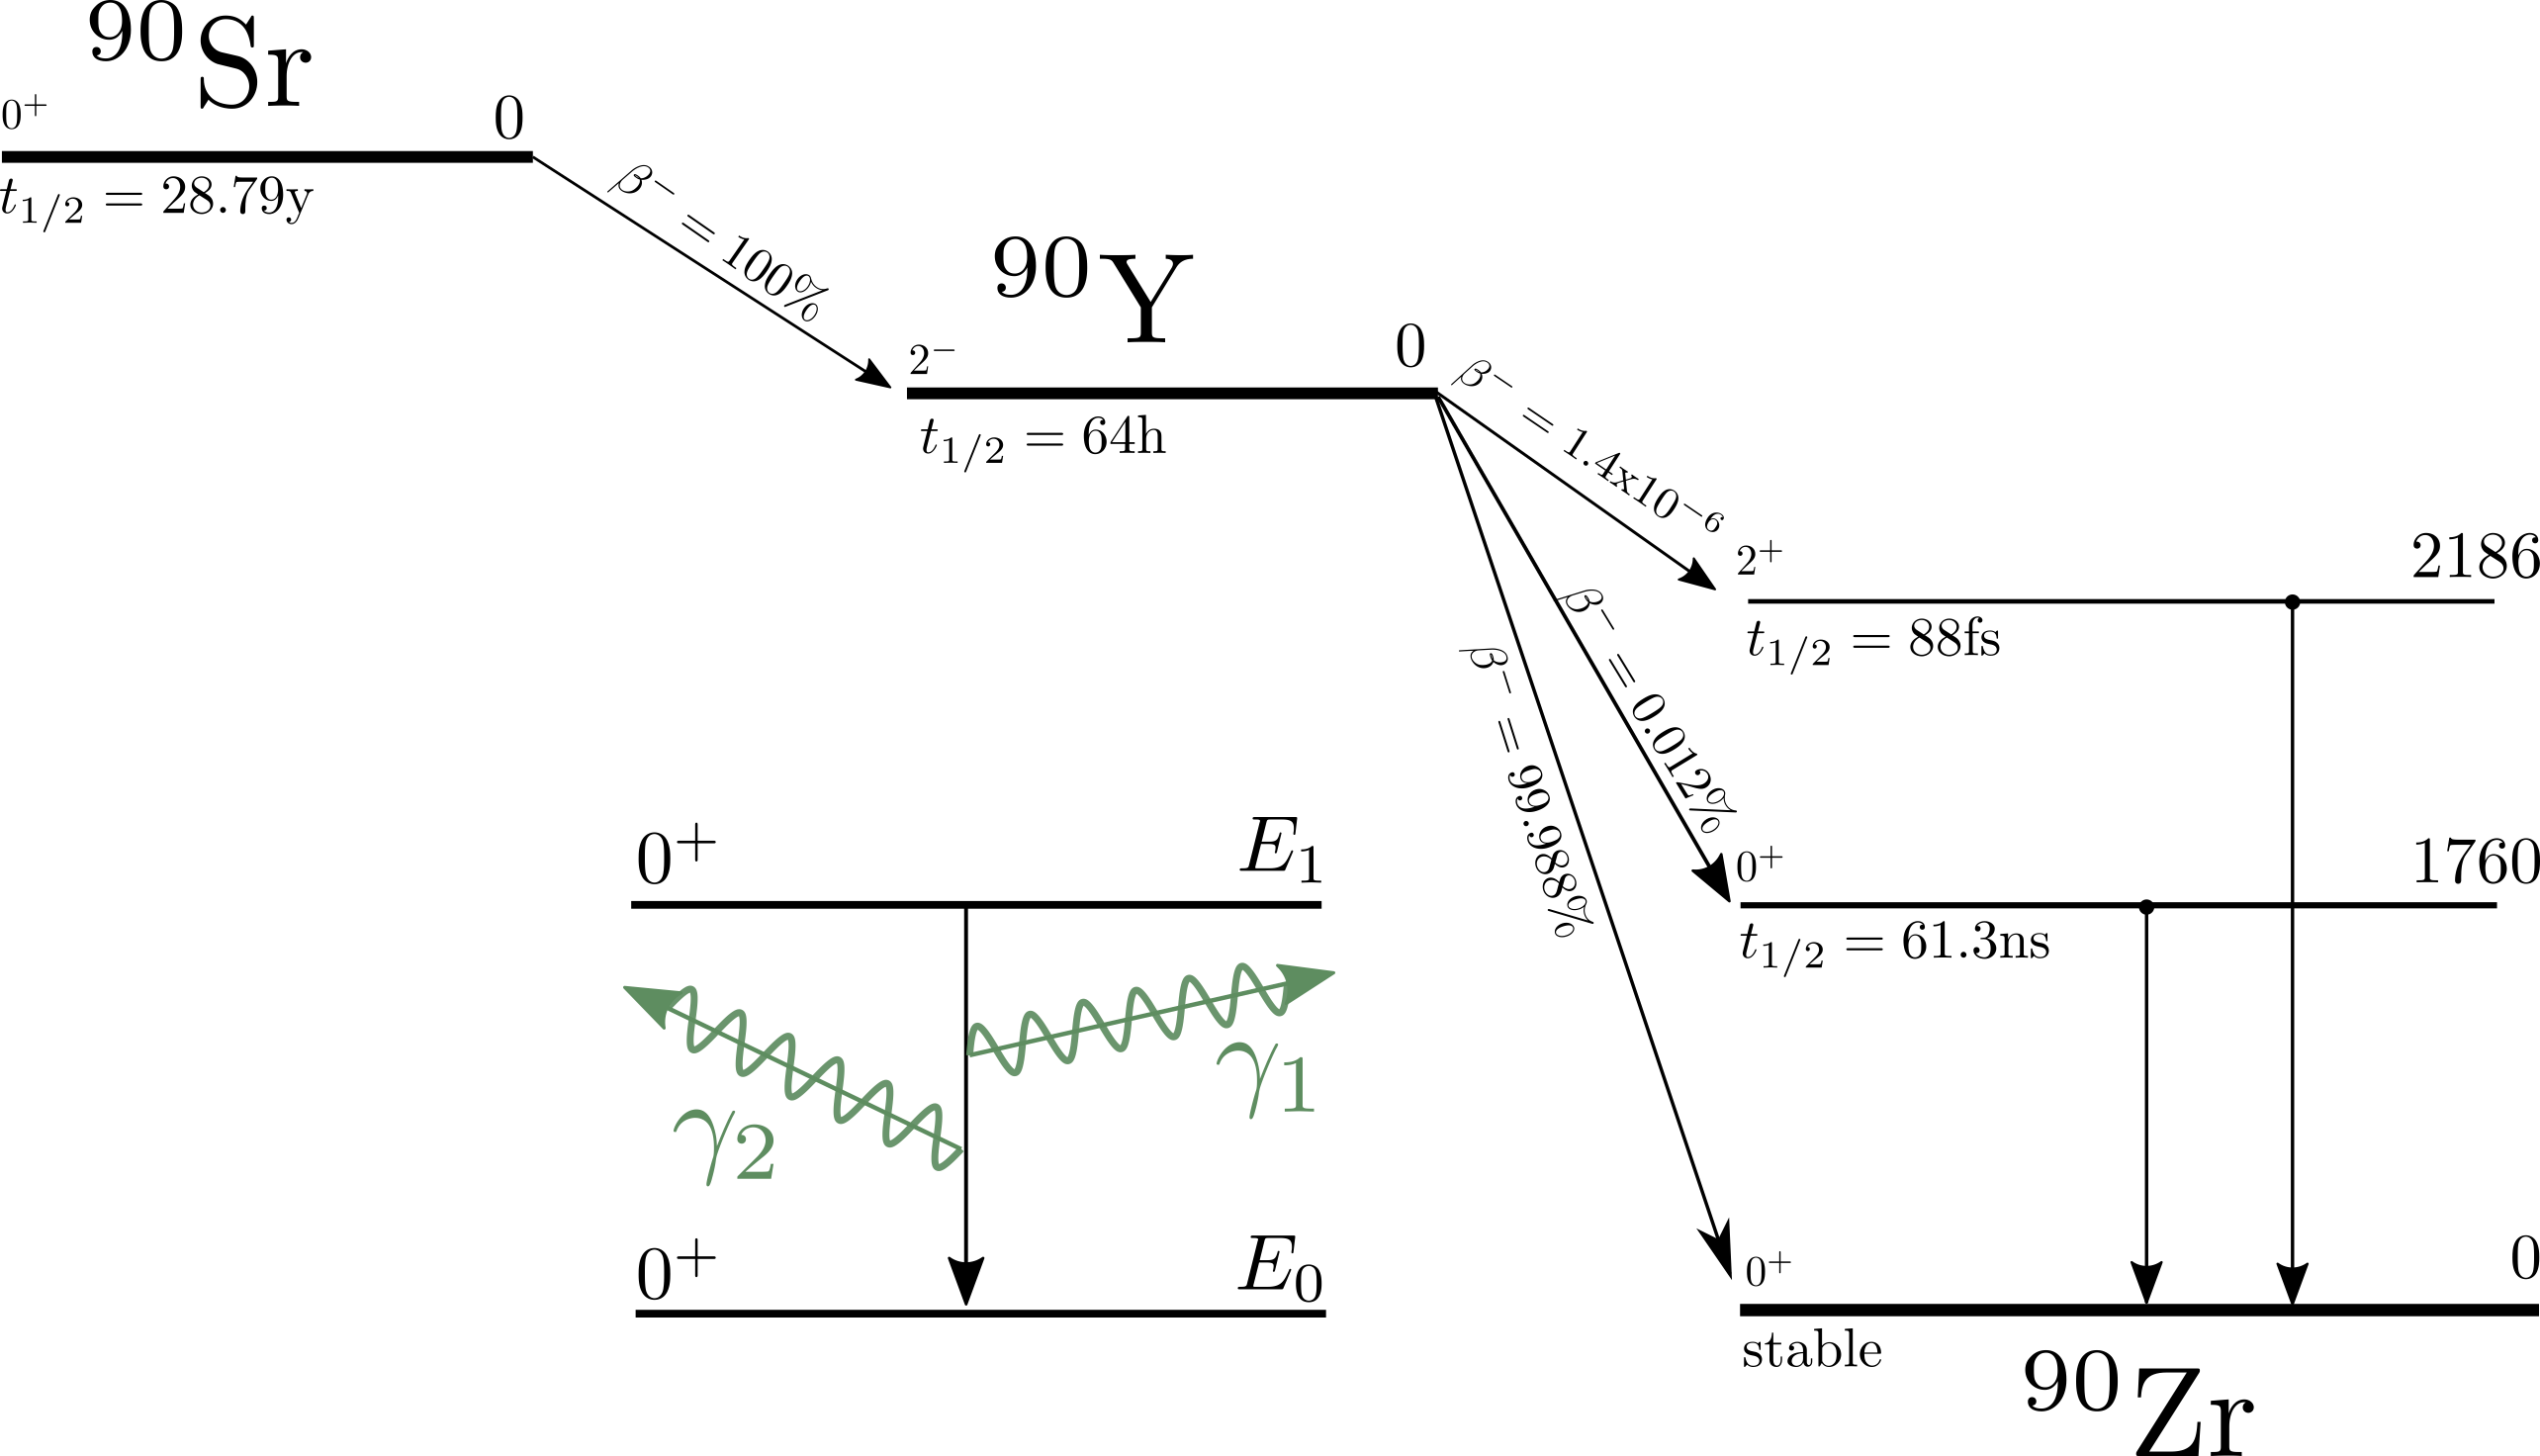
\includegraphics[width=0.95\textwidth]{decay_scheme_with_twophoton.png}
  \caption{Decay scheme of a $^{90}$Sr source with the insert schematically detailing non-competitive two-photon decay. All energies are in keV.}
  \label{fig:decay_scheme_with_twophoton}
\end{figure}

%------------------------------------------
\subsection{Sum Spectrum}
\label{sec:sum_spectrum}
%------------------------------------------

The two photons released during a two-photon decay event sum to the total energy of the transition, meaning the full energy of the transition should show up as a peak in a sum spectrum. 
A sum spectrum is generated by adding the energies of two incident photons together and recording their resultant sum in a histogram.
This is similar to the GRIFFIN addback algorithm, where the energy of all events detected within a single clover are summed together, but does not restrict the sum to singles events within the same clover; but rather, sums events together that were registered in different crystals regardless of if they were in the same clover of not. 
\ref{fig:singles_vs_sum_spectrum} shows the difference between a singles $\gamma$-ray energy spectrum and a sum spectrum.

\begin{figure}[htbp]
  \centering
  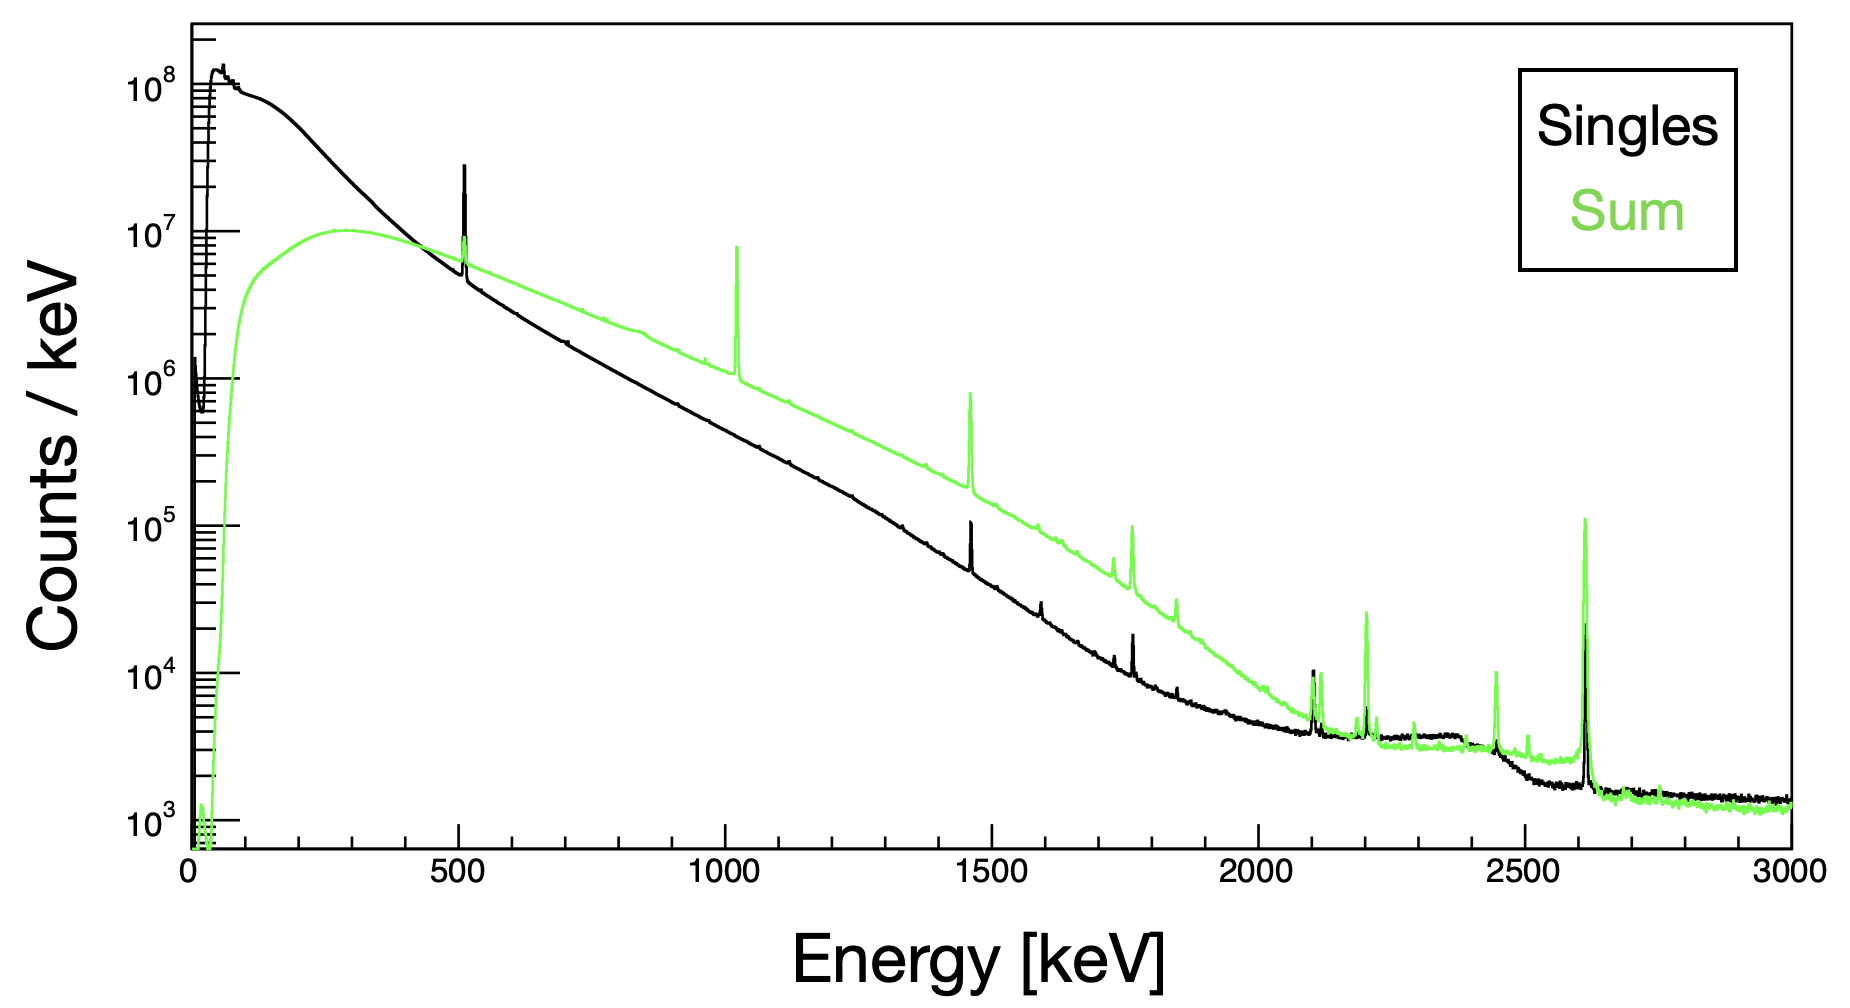
\includegraphics[width=0.95\textwidth]{singles_vs_sum_spectrum.png}
  \caption{Comparison of singles (black) and sum (green) spectra for 506 hours of $^{90}$Sr source collection.}
  \label{fig:singles_vs_sum_spectrum}
\end{figure}

%------------------------------------------
\subsection{First Test - November 2017}
%------------------------------------------
The first attempt at measuring two-photon decay with GRIFFIN occurred in November 2017 using a 19 MBq $^{90}$Sr source already present at TRIUMF and was used to evaluate the feasibility of measuring two-photon transitions and assess the background level in the array.
The $^{90}$Sr source was placed in the center of a DELRIN sphere to suppress the Bremsstrahlung radiation from the emitted beta particles, and the DELRIN sphere was screwed onto a PEEK source holder rod locking it into position (\ref{fig:source_support_picture}).
The source was aligned to the centre of the array using a laser pointer mounted to the upstream beamline.
All sixteen GRIFFIN clovers were present in the array in high-efficiency mode and the $^{90}$Sr puck source was roughly aligned to the centre of the array using a source holder.
X-ray absorbers, composed of 0.1 mm layer of Tantalum (Ta), 0.25 mm layer of Tin (Sn), and 0.25 mm layer of Copper (Cu), were placed in front of the clover faces with the Cu layer facing the clover to reduce the low energy x-ray flux on the HPGe clovers.
No BGO suppression shields were present for this data collection. 
DAQ rates are detailed in \ref{tab:daq_rates}.

\begin{figure}[htbp]
  \centering
  \includegraphics[width=0.95\textwidth]{source_support_picture.png}
  \caption{$^{90}$Sr source centred in GRIFFIN. The source is surrounded by a DELRIN sphere and the sphere is held into place with a PEEK support rod. The X-ray absorbers in the downstream opening to the right of the source holder were placed on the front face of the HPGe detectors during this test.}
  \label{fig:source_support_picture}
\end{figure}


\begin{table}[]
  \centering
  \begin{tabular}{cccccc}
                    & Source                  & Source Activity & Crystal Rate & Total Array Rate & Data Rate \\ \hline
  \textbf{Nov 2017} & $^{90}$Sr - commercial  & ~19 MBq         & 15-22 kHz    & 625 kHz          & 26.6 MB/s \\ \hline
  \textbf{Jul 2018} & $^{90}$Sr - commercial  & ~19 MBq         & 4-8 kHz      & 305 kHz          & 12.9 MB/s \\ \hline
  \textbf{Dec 2019} & $^{90}$Sr - custom      & ~19 MBq         & 2-2.5 kHz    & 20 kHz           & 1.0 MB/s  \\
                    & Room Background         & -               & 200 Hz       & -                & 0.2 MB/s  \\ \hline
  \end{tabular}
  \caption{DAQ data rates for the three data collections}
  \label{tab:daq_rates}
\end{table}

\ref{fig:sum_spectrum_jul2017} shows the sum spectrum generated from this data collection.
There is a peak in the two-photon region of interest with a centroid of 1764 keV from $^{214}$Bi decay masking any possible two-photon peak.
Furthermore, the presence of two peaks, at 57 and 65 keV respectively, indicate the presence of tungsten in the ceramic backing of the button source.
This flouresce causes the detectors directly behind the source (where the x-ray radiation shine is the strongest) to have a higher count rate than the detectors on the opposite side of the array and random summing with these x-rays causes a significant background in the sum spectrum that must be reduced to observe a two-photon peak. 
With no way to veto Compton scatters and the large x-ray flux coming from the source no two-photon peak could be observed with this source.

\begin{figure}[htbp]
  \centering
  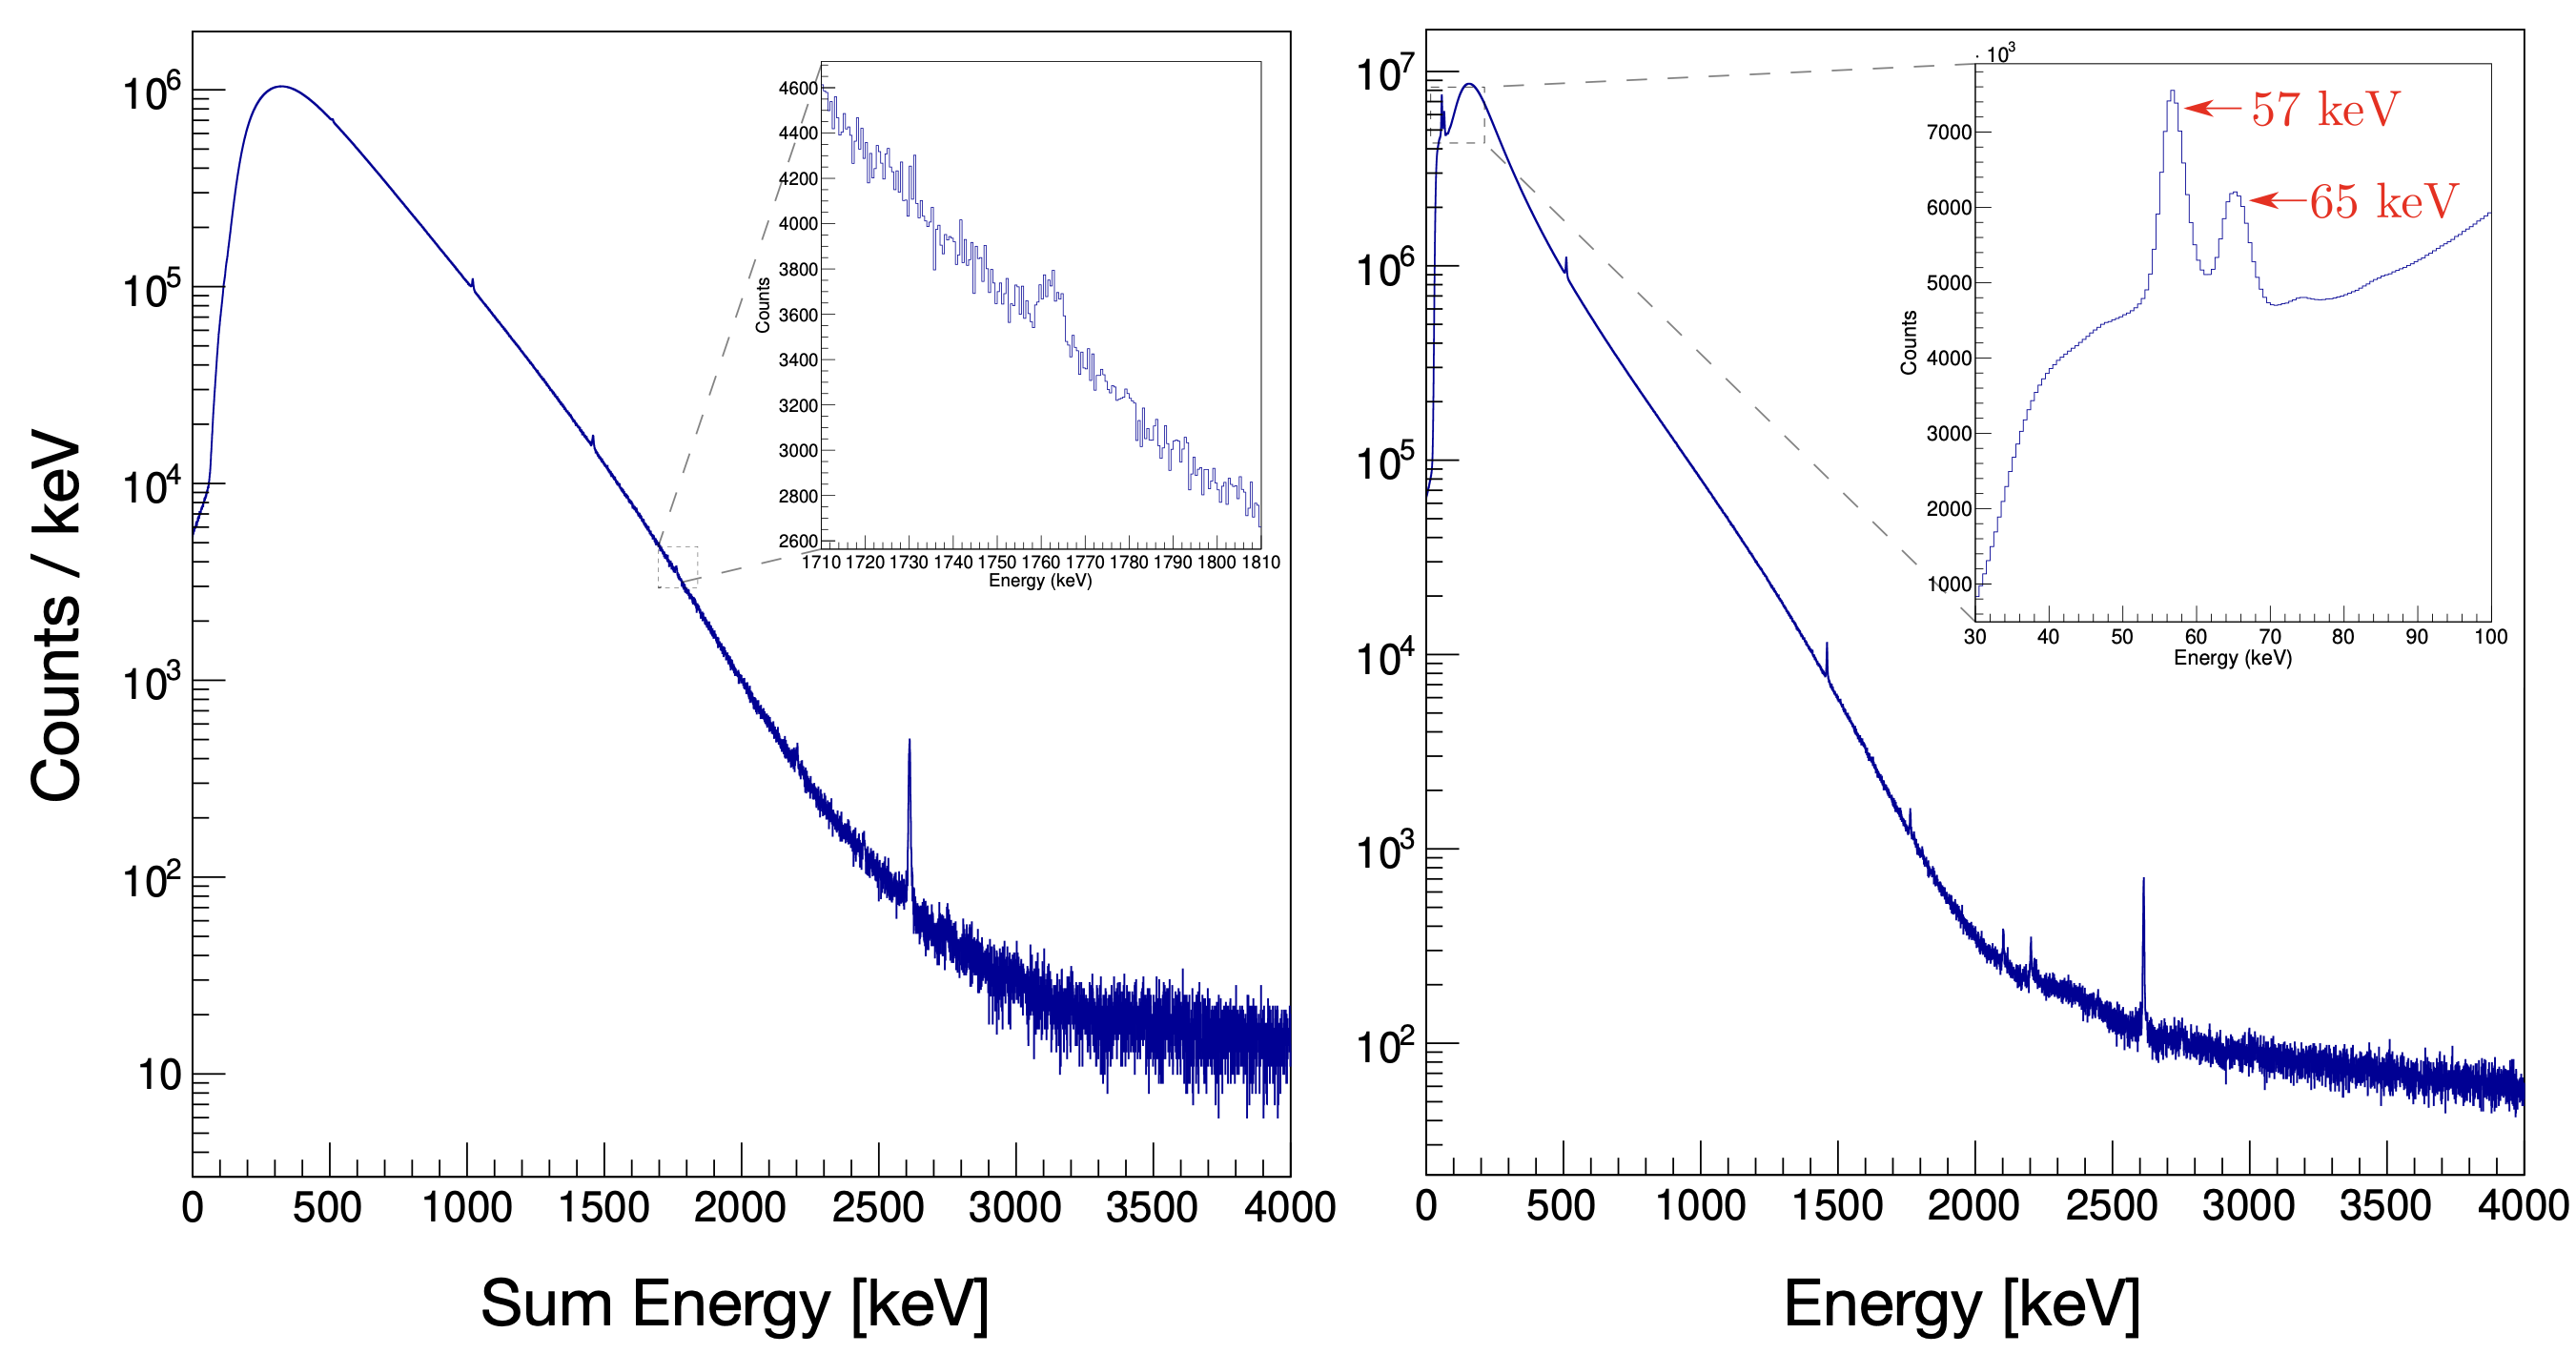
\includegraphics[width=0.95\textwidth]{first_collection_sum_spectrum.png}
  \caption{Sum spectrum from 10 hours of a ~19 MBq $^{90}$Sr source.
    \textit{Left:} Sum spectrum with the insert showing the region around 1760 keV. There is a peak, but it is from the 1764 keV $^{214}$Bi $\beta$-decay room background.
    \textit{Right:} $\gamma$-ray singles energy spectrum with the insert showing the 57 and 65 keV x-ray flouresce lines from the tungsten dopant in the source holder ceramic backing.
  }
  \label{fig:sum_spectrum_jul2017}
\end{figure}

%------------------------------------------
\subsection{Second Test - July 2018}
%------------------------------------------
Between the November 2017 and this data collection in July 2018 a full complement of BGO Compton suppression shields were installed on GRIFFIN providing an increase in the signal-to-noise ratio of the array.
The DELRIN source holder was modified to no longer screw onto the DELRIN support structure, instead the sphere now sat on a bronze hoop allowing the radiation shine from the ceramic backing of the $^{90}$Sr source to be directed upstream and therefore improve the spectral quality for the other 12 clovers.
\ref{fig:source_holder_jul2018} shows the modified source holder.

\begin{figure}[htbp]
  \centering
  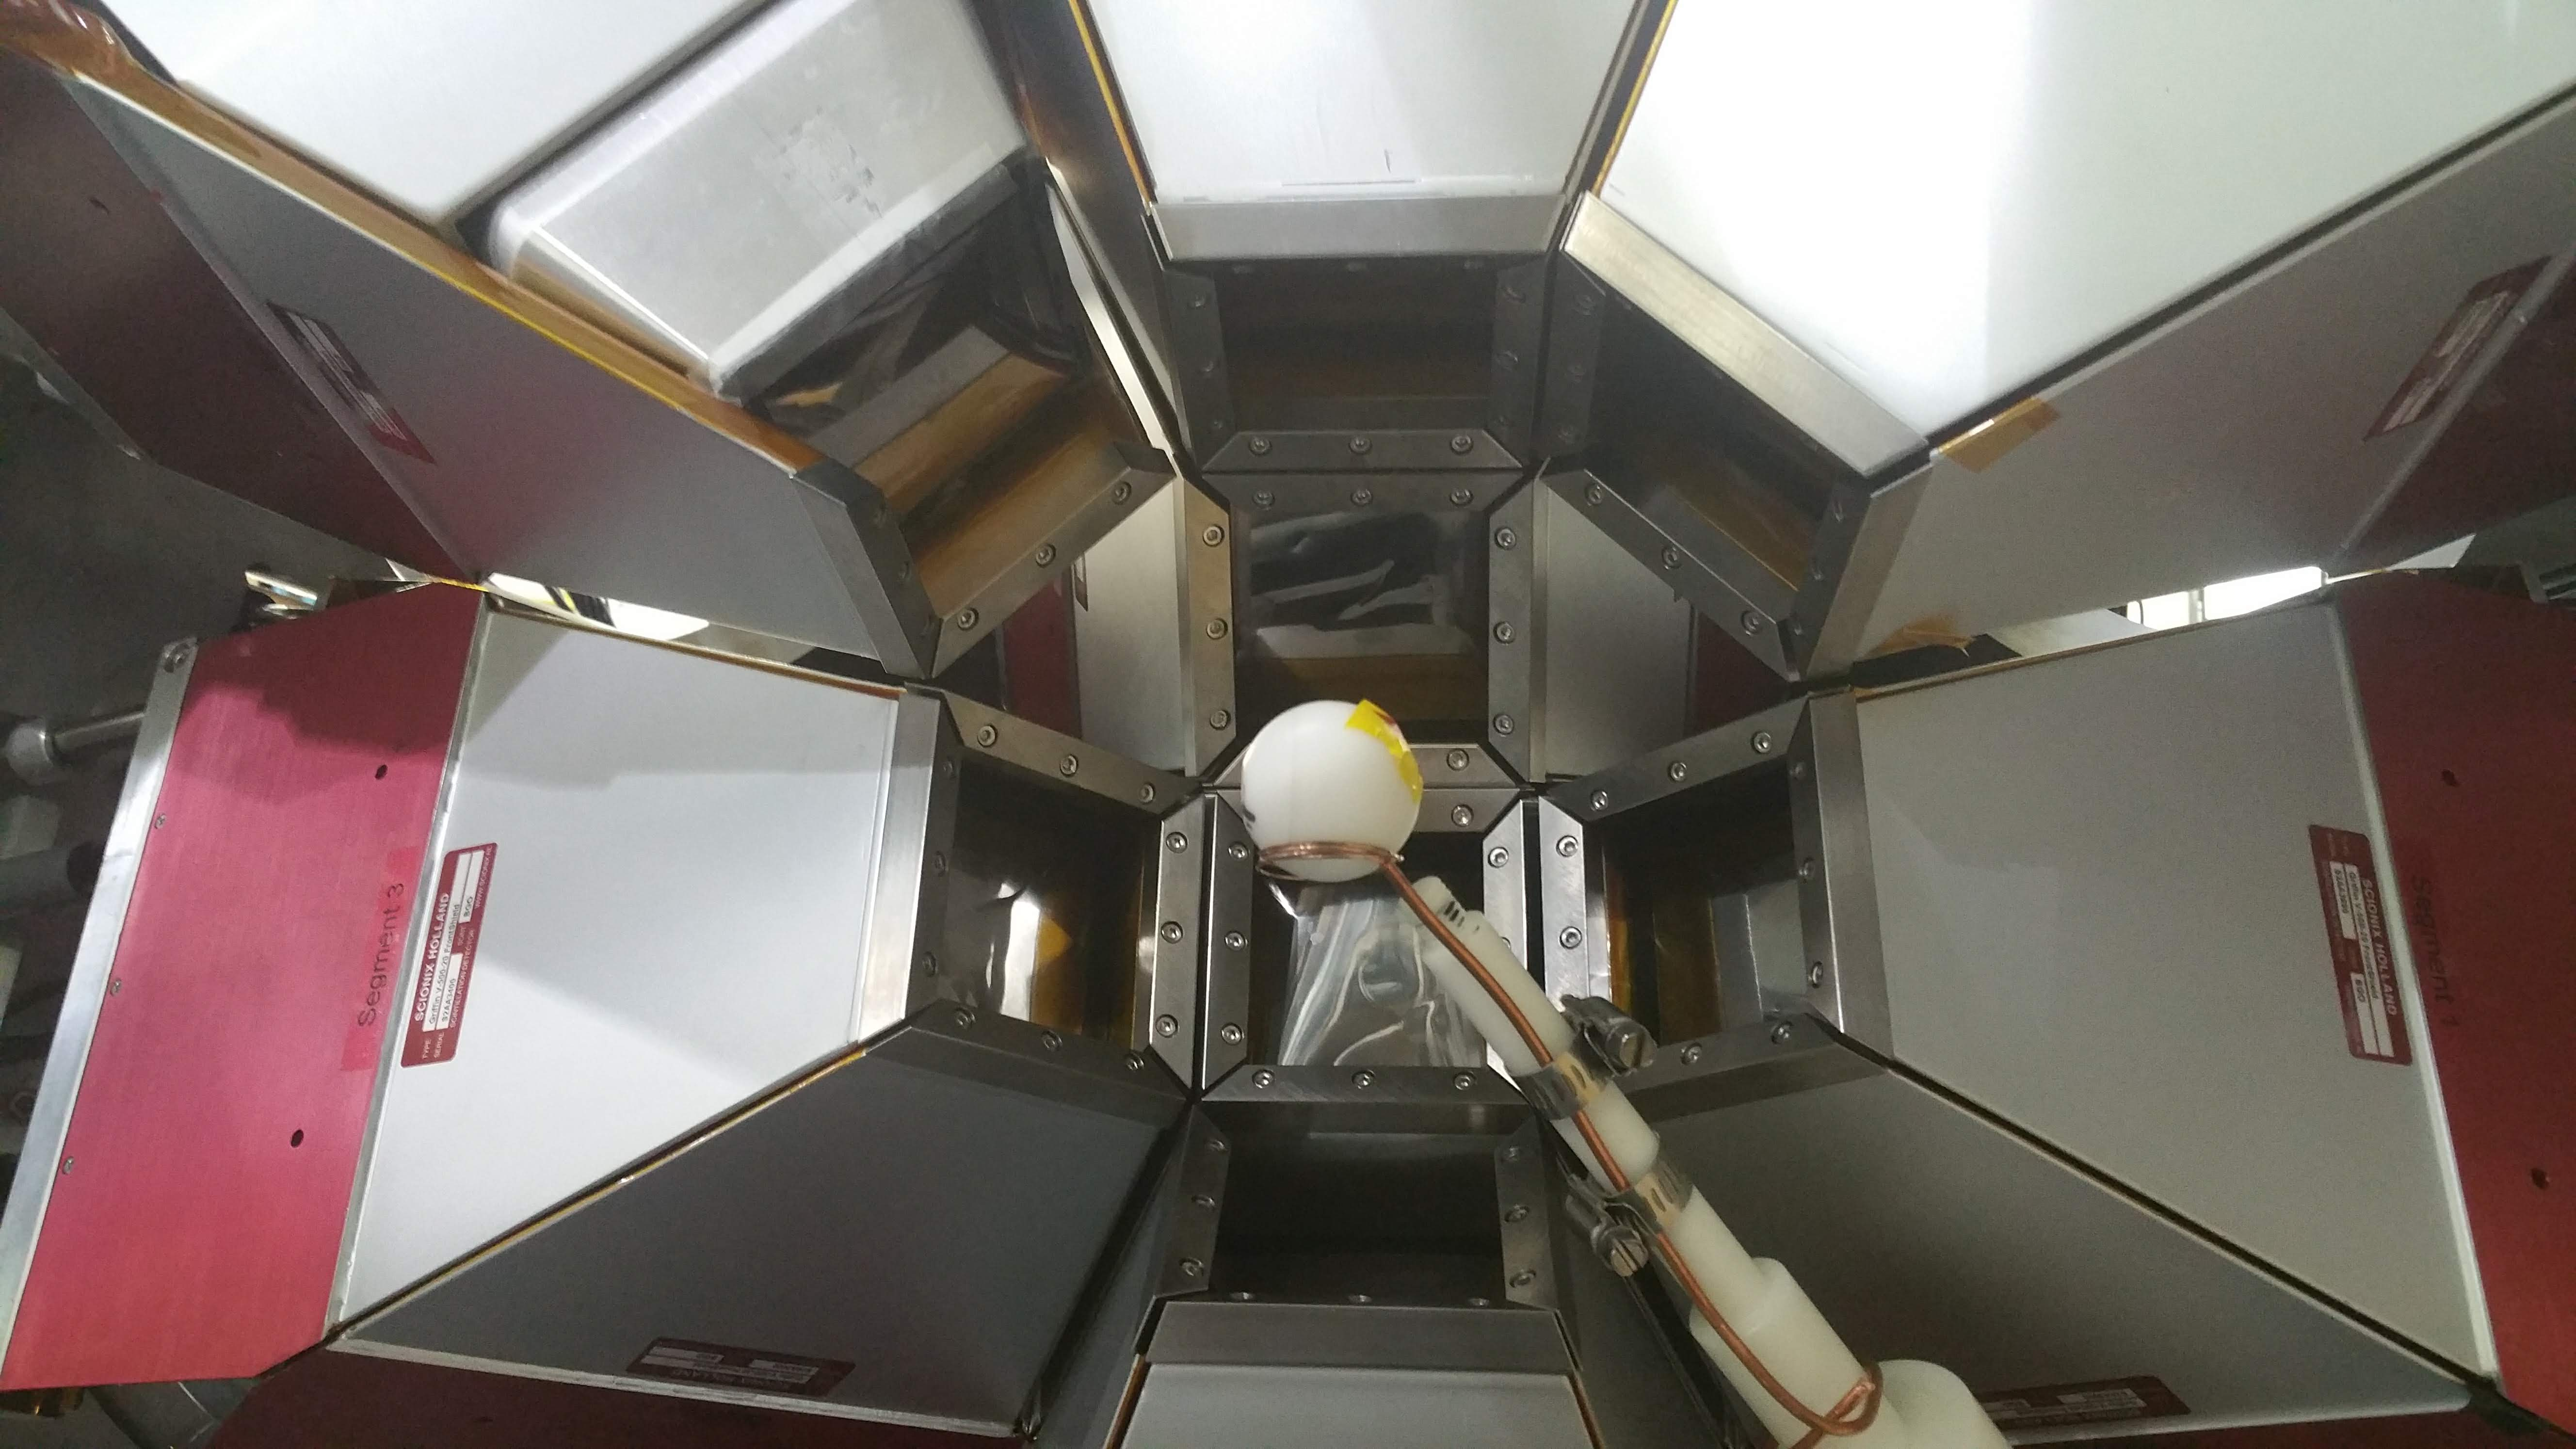
\includegraphics[width=0.95\textwidth]{jul2018_sourceholder.jpg}
  \caption{DELRIN source holder containing the $^{90}Sr$ source and mounted on the modified support structure. The bronze ring allows the source holder to be rotated to direct the radiation shine from the ceramic backing to be directed upstream.}
  \label{fig:source_holder_jul2018}
\end{figure}

\ref{fig:sum_spectrum_jul2018} is the sum spectrum generated from this dataset. 
The tungsten x-rays are no longer present and the 1764 keV peak is suppressed. 
Despite the addition of BGO-suppression shields and the modified source holder the Bremsstrahlung radiation from the interaction of the emitted betas and the source ceramic pellet created too much background and two-photon signals could not be distinguished.
The clovers directly behind the pellet had a count rate twice that of the others, 8 kHz vs 4 kHz (See Table~\ref{tab:daq_rates}), thus suggesting a new source was required to make an observation.

\begin{figure}[htbp]
  \centering
  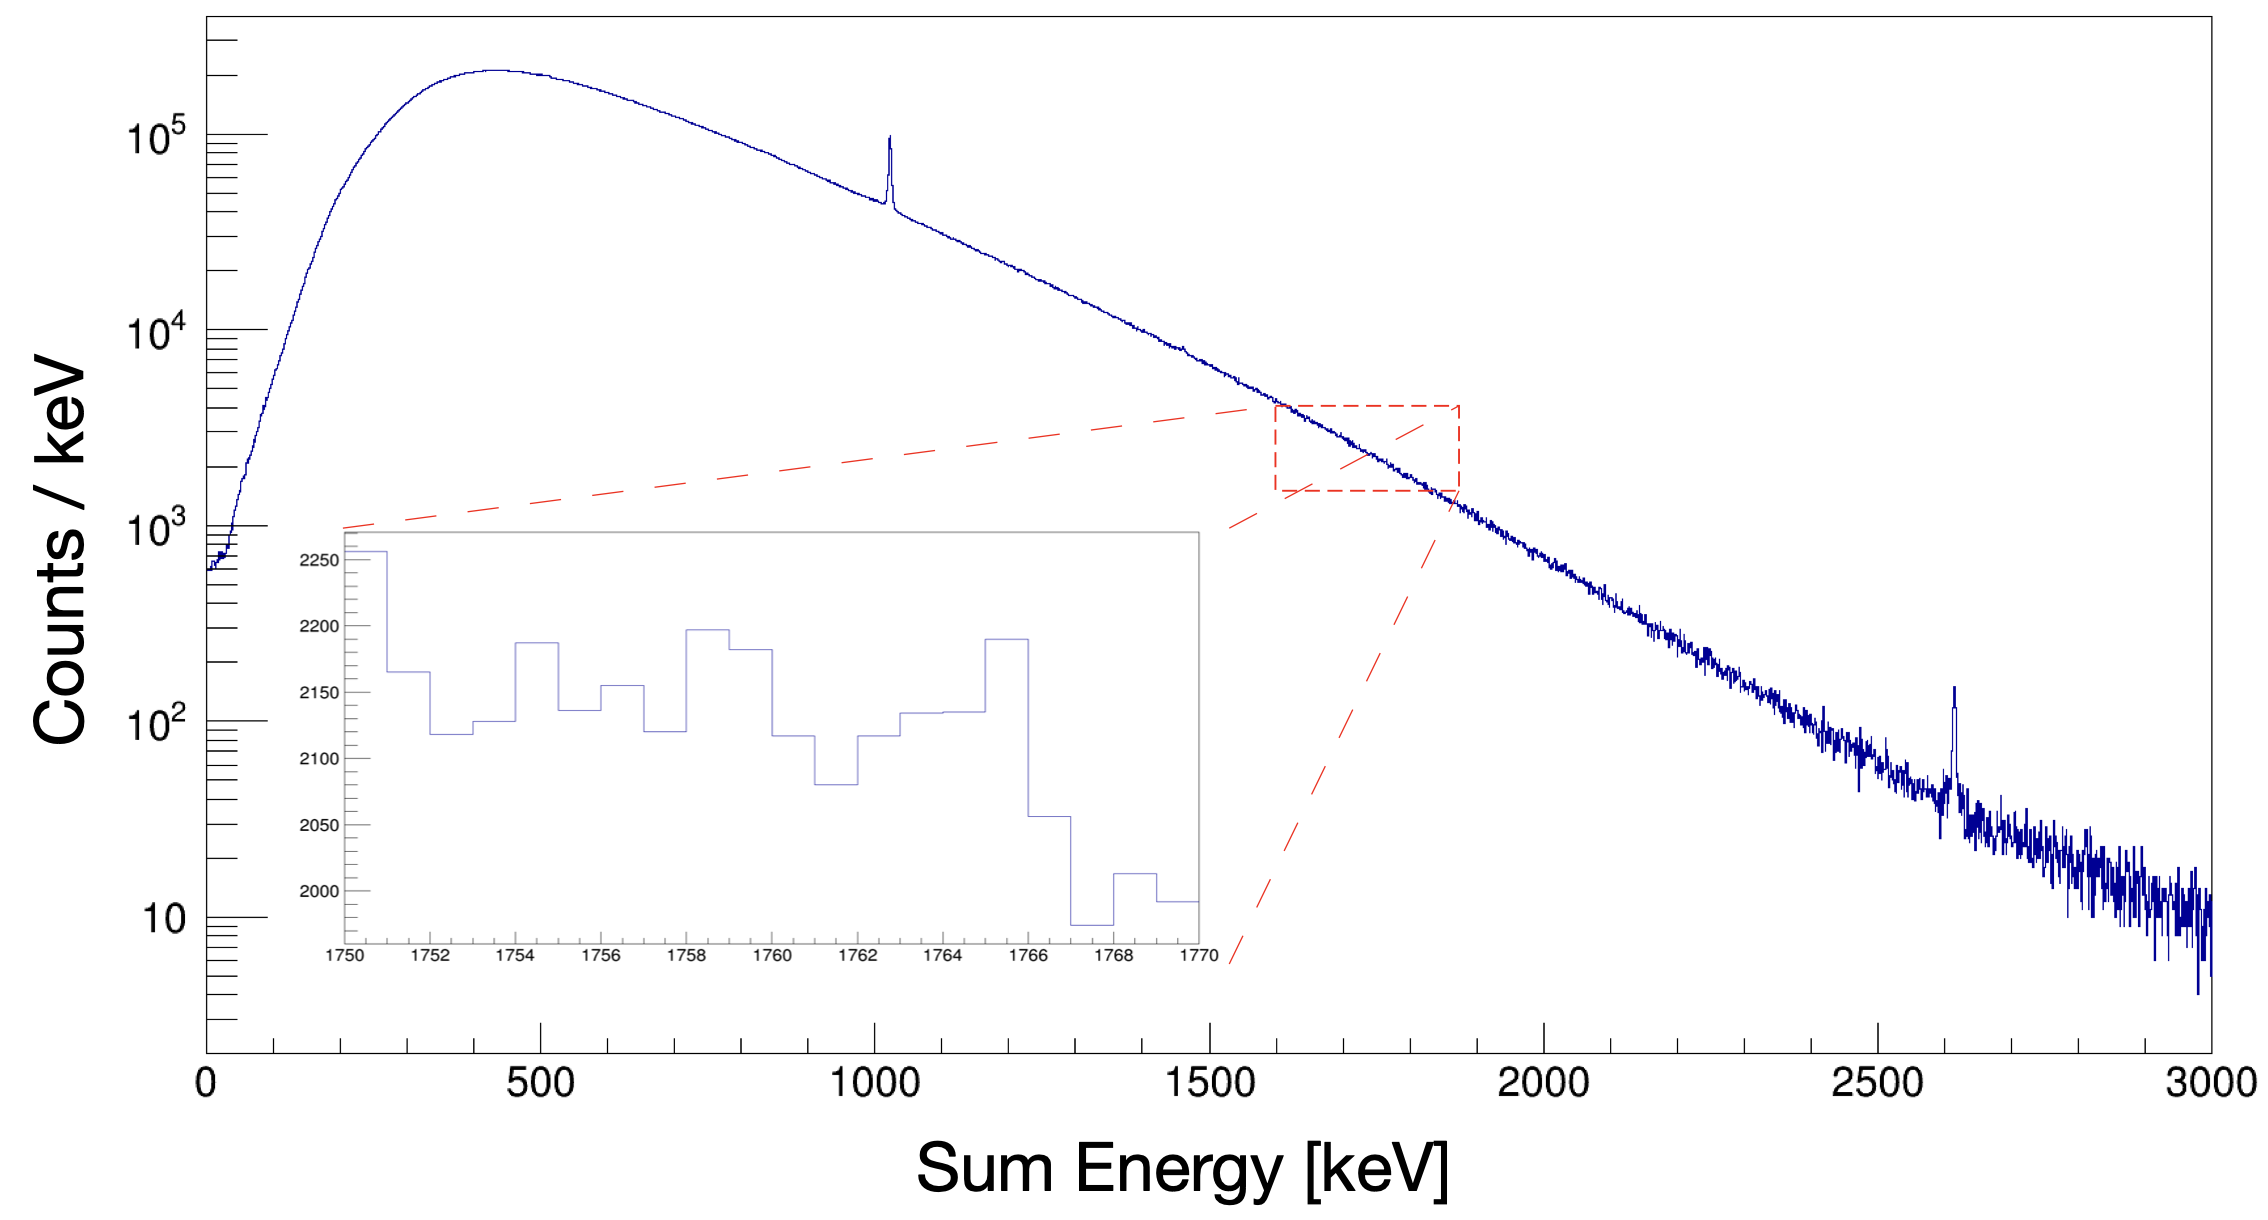
\includegraphics[width=0.95\textwidth]{jul2018_sum_spectrum.png}
  \caption{Sum spectrum from 10 hours of a ~19 mbq $^{90}$Sr source using BGO-suppression shields and a modified source holder. The tungsten x-rays are no longer present, but no two-photon peak is visible. The Bremsstrahlung radiation from the ceramic pellet is still too high to observe a two-photon transition.}
  \label{fig:sum_spectrum_jul2018}
\end{figure}

%------------------------------------------
\subsection{Third Test - December 2019}
%------------------------------------------

Prior to this data collection the $^{90}$Sr source had the activity mounted on an industrial ceramic backing causing a significant low-energy background that obscured any two-photon peak.
The high beta activity of the source caused the Tungsten dopant in the ceramic to flouresce x-rays, of characteristic energy 57 and 65 keV, measured primarily in detectors directly behind the ceramic backing of the source and doubling the count rate compared to the rest of the array. 
Furthermore, the ceramic and the bronze source holder were made of sufficiently high-Z materials such that the Bremsstrahlung radiation from the interaction of the betas released from the source masked any two-photon signal that GRIFFIN could measure.
The high flux of low-energy Bremsstrahlung radiation through the array caused many spurious coincidences, a Bremsstrahlung photon summing with another photon from any source, that raised the background level of the sum spectrum to mask the 1760 keV two-photo sum peak.

To remove the tungsten x-rays and reduce the Bremsstrahlung radiation a new custom source was fabricated where the $^{90}$Sr activity was deposited directly in the centre of a DELRIN (polyoxymethylene) sphere.
A commercially obtained 20 MBq liquid Strontium Chloride, dissolved in 0.1M HCL, source was purchased and the source was evaporated into the centre of a DELRIN sphere, which was then sealed by TRIUMF radiochemist Valery Radchenko.
\ref{fig:source_holder} shows the source holder pre-source evaporation.
Since there is no high-Z material in the source holder the Bremsstrahlung radiation is strongly reduced compared to the original source.

% TODO Add picture

\begin{figure}[htbp]
  \centering
  \subfloat{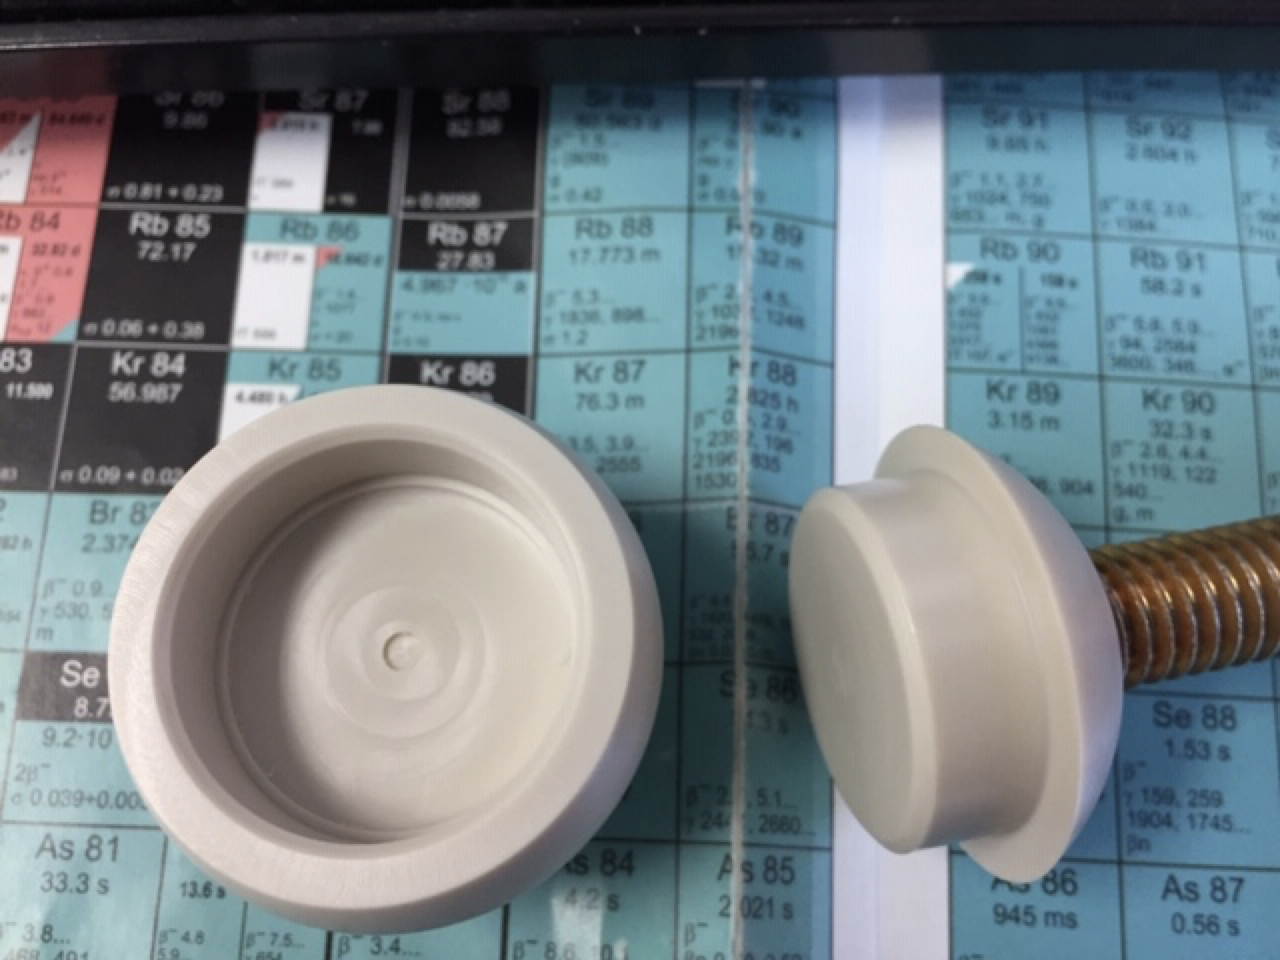
\includegraphics[height=5cm]{source_holder_open.png}}
  \quad
  \subfloat{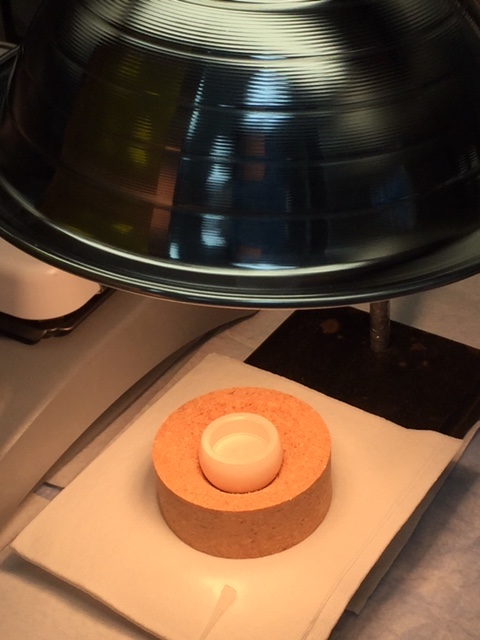
\includegraphics[height=5cm]{custom_source_evaporation.JPG}}
  \quad
  \subfloat{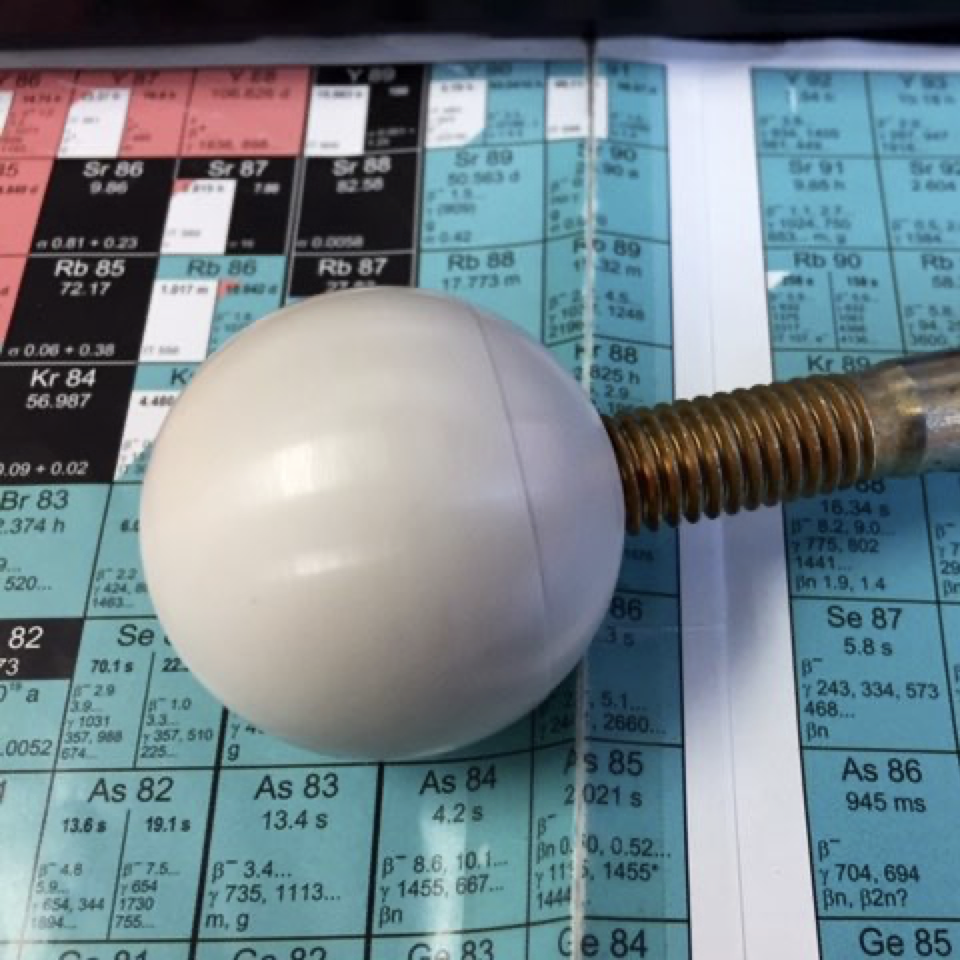
\includegraphics[height=5cm]{source_holder_closed.png}}
  \caption{
    \textit{Left:} DELRIN source holder before $^{90}$Sr activity deposit. The activity will be deposited in the centre of the larger section via evaporation of a Strontium Chloride solution.
    \textit{Middle:} Strontium Chloride solution being evaporated onto the centre of the DELRIN sphere.
    \textit{Right:} DELRIN source holder with both halves closed together.
  }
  \label{fig:source_holder}
\end{figure}

A PEEK (polyetheretherketone) source holder was fabricated to hold the sphere containing the $^{90}$Sr activity in the centre of the array and the Ta/Sn/Cu X-ray absorbers were placed in the open faces of the GRIFFIN rhombicuboctahedron to increase the passive shielding of the array. This configuration is shown in the left panel of Figure~\ref{fig:source_holder_in_griffin}. The source holder was aligned using a laser point placed on the upstream beamline, shown in the right panel of Figure~\ref{fig:source_holder_in_griffin}.

\begin{figure}[htbp]
  \centering
  \subfloat{\includegraphics[height=7cm]{custom_90Sr_source.jpg}}
  \quad
  \subfloat{\includegraphics[height=7cm]{beamline_xray_absorbers.png}}
  \caption{
    \textit{Left:} Photograph of $^{90}$Sr source and source holder aligned to the centre of GRIFFIN. Ta/Sn/Cu X-ray absorbers were placed in the opening faces of the GRIFFIN rhombicuboctahedron to help reduce room background and increase passive shielding.
    \textit{Right:} Photograph of $^{90}$Sr holder looking upstream. The red arrow points to the laser pointer used to align the source sphere.
  }
  \label{fig:source_holder_in_griffin}
\end{figure}

% todo: add comparision plot of cyclotron on vs off?
Unlike the previous data collections this dataset was taking during the TRIUMF annual shutdown, when TRIUMF shuts down the main cyclotron and RIB production for maintenance and development, to reduce the neutron flux through the experimental hall. Data collection started in late December 2020 and continued through January 2021 for a total of 500 hours of source data and 300 hours of room background. The HPGe crystals were counting at 2-2.5 kHz during the source collection and 200 Hz during the room background collection, with a DAQ rate of 1 MB/s and 0.2 MB/s respectively.

The new custom source holder allowed for greater peak fidelity and completely removed the tungsten fluorescent x-rays.
\ref{fig:dec2020_gamma_singles} is the gamma singles, using HPGe crystal energies rather than addback, energy spectrum from 506 hours of data collection.

\begin{figure}[htbp]
  \centering
  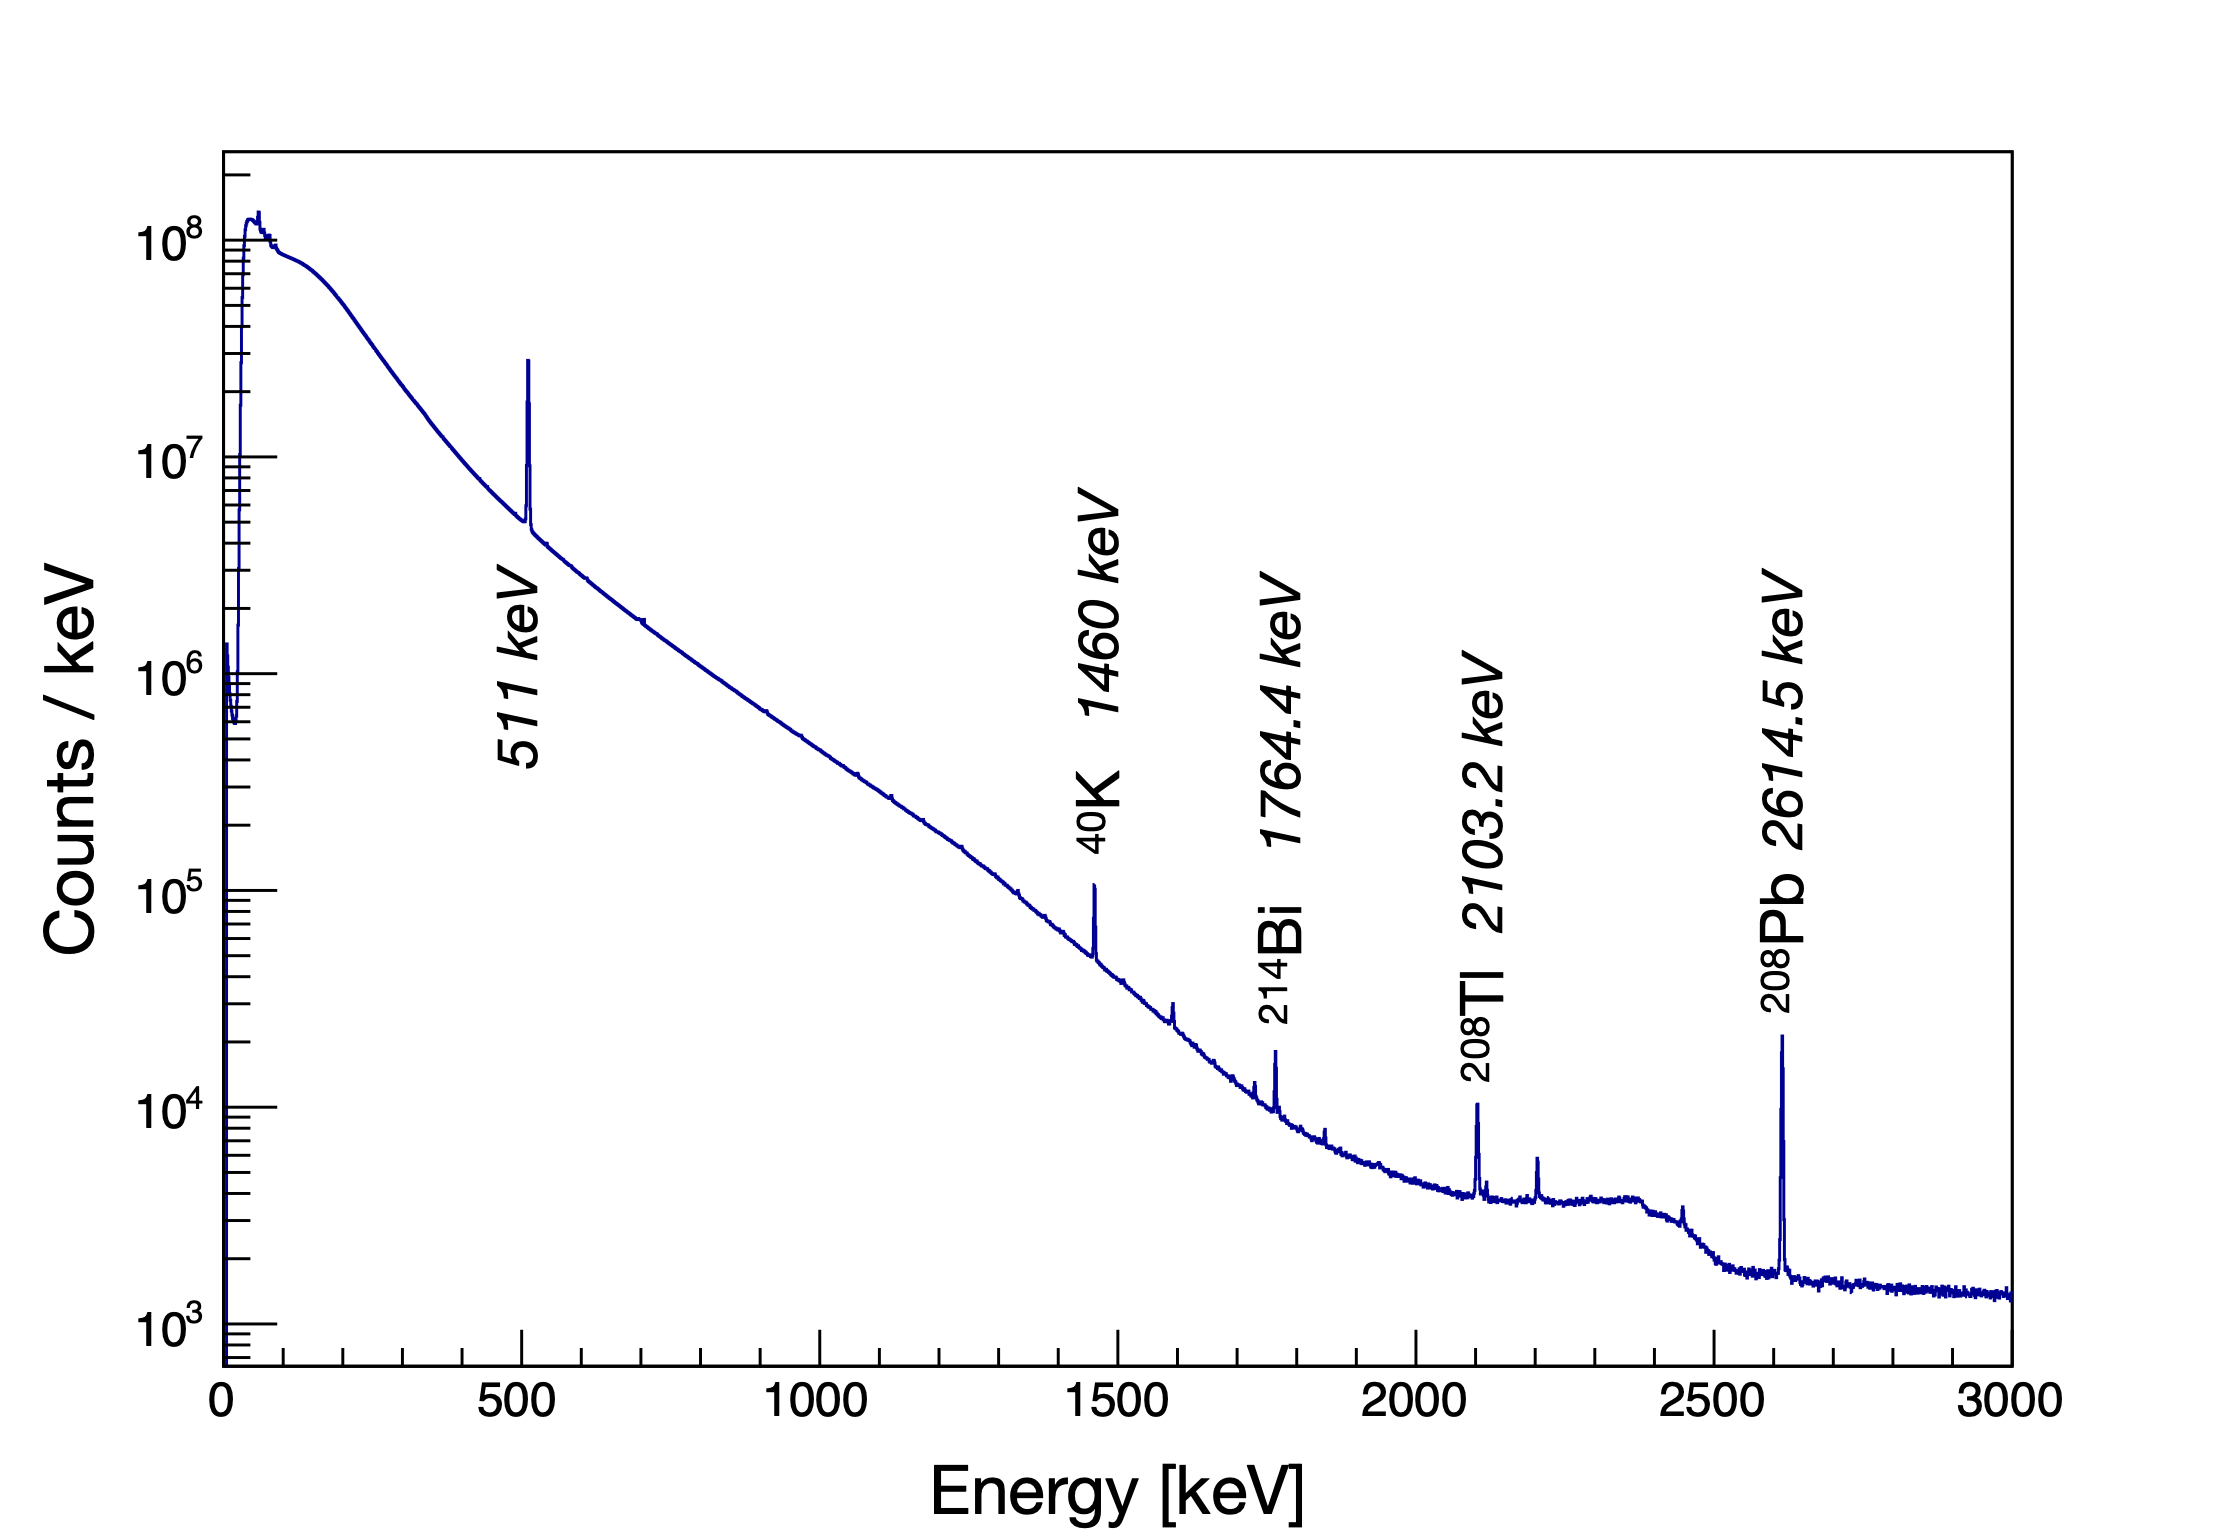
\includegraphics[width=0.95\textwidth]{dec2020_gamma_singles.png}
  \caption{$\gamma$-ray singles energy spectrum from 506 hours of $^{90}$Sr source data collection. Prominent room background peaks have been labeled.}
  \label{fig:dec2020_gamma_singles}
\end{figure}

The new source reduced the Bremsstrahlung radiation present in the previous data collections and reduced the background in the sum spectrum to sufficiently low levels to see a two-photon peak.
\ref{fig:sum_spectrum_dec2019} shows the sum spectrum from this data collection after a statistical background subtraction has been performed.

\begin{figure}[htbp]
  \centering
  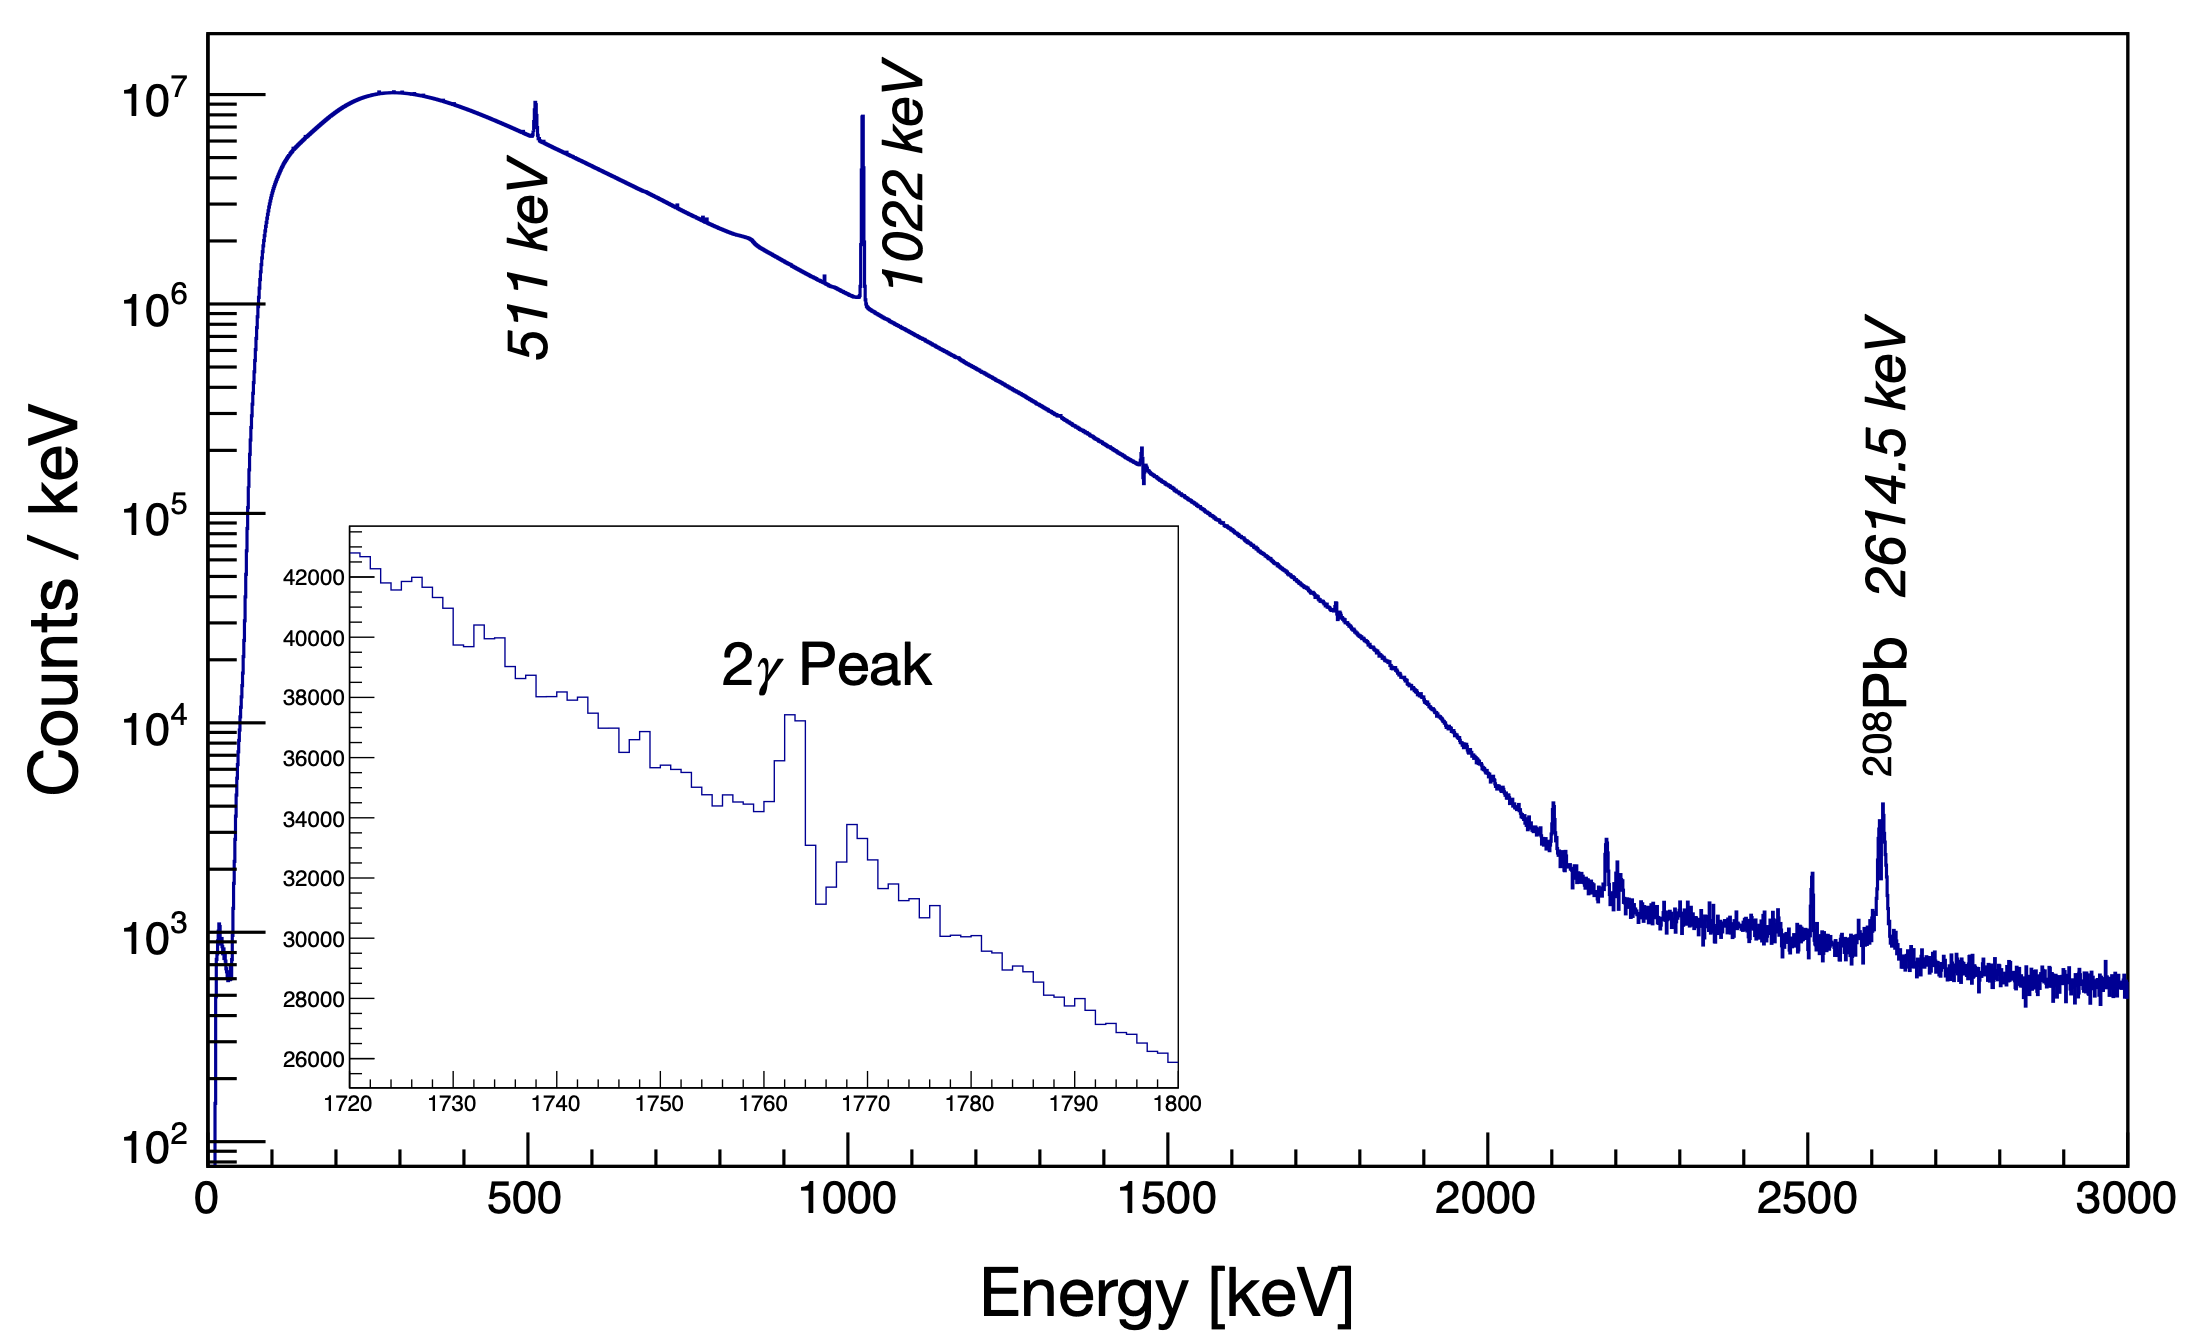
\includegraphics[width=0.95\textwidth]{sum_spectrum_dec2019.png}
  \caption{Room background subtracted $\gamma$-ray energy sum spectrum from 506 hours of $^{90}$Sr source and 300 hours of room background data. Major peaks are labeled and only events of multiplicity two were used to fill the histogram. \textit{Insert:} Focus on the region where the 1760 keV two-photon peak is expected. Here the statistical background subtraction of the 1764 keV peak from $^{214}$Bi decay can be seen.}
  \label{fig:sum_spectrum_dec2019}
\end{figure}

%------------------------------------------
\subsection{Further Analysis}
\label{sec:further_analysis}
%------------------------------------------
Since evidence of a two-photon transition can be seen in \ref{fig:sum_spectrum_dec2019}, the following sections detail further analyses performed on the December 2019 data.

%------------------------------------------
\subsubsection{Angular Matrices}
\label{sec:angular_matrices}
%------------------------------------------

The angular correlation between the two photons composing nuclear two-photon decay is a powerful tool for assigning the transition polarizability and susceptibility of the excited state, as described by equation~\ref{eqn:angular-distribution}.
This angular correlation is distinct to two-photon decay and can be used as a condition to isolate two-photon decays from other multiplicity two events; such as internal and external Compton-scattering.
Both internal and external Compton-scattering are a single photon that doesn't deposit its full energy in a single crystal but rather scatters into another crystal and deposits the remaining energy, making it a multiplicity two event and a peak in the sum spectrum.
The difference between internal and external is the source of the photon: internal originates from the centre of the array, for example a $^{207}$Bi source; and external originates from outside the array, most commonly room background $\gamma$-rays as discussed in Section~\ref{sec:room_background}.
Each of the three different cases, two-photon decay, internal and external Compton-scatters, all have a distinct angular correlation matrix.
\ref{fig:external_compton_scatter_schematic}, \ref{fig:internal_compton_scatter_schematic}, and \ref{fig:two_photon_angular_schematic} show the difference between the three angular matrices

\begin{figure}[htbp]
    \centering
    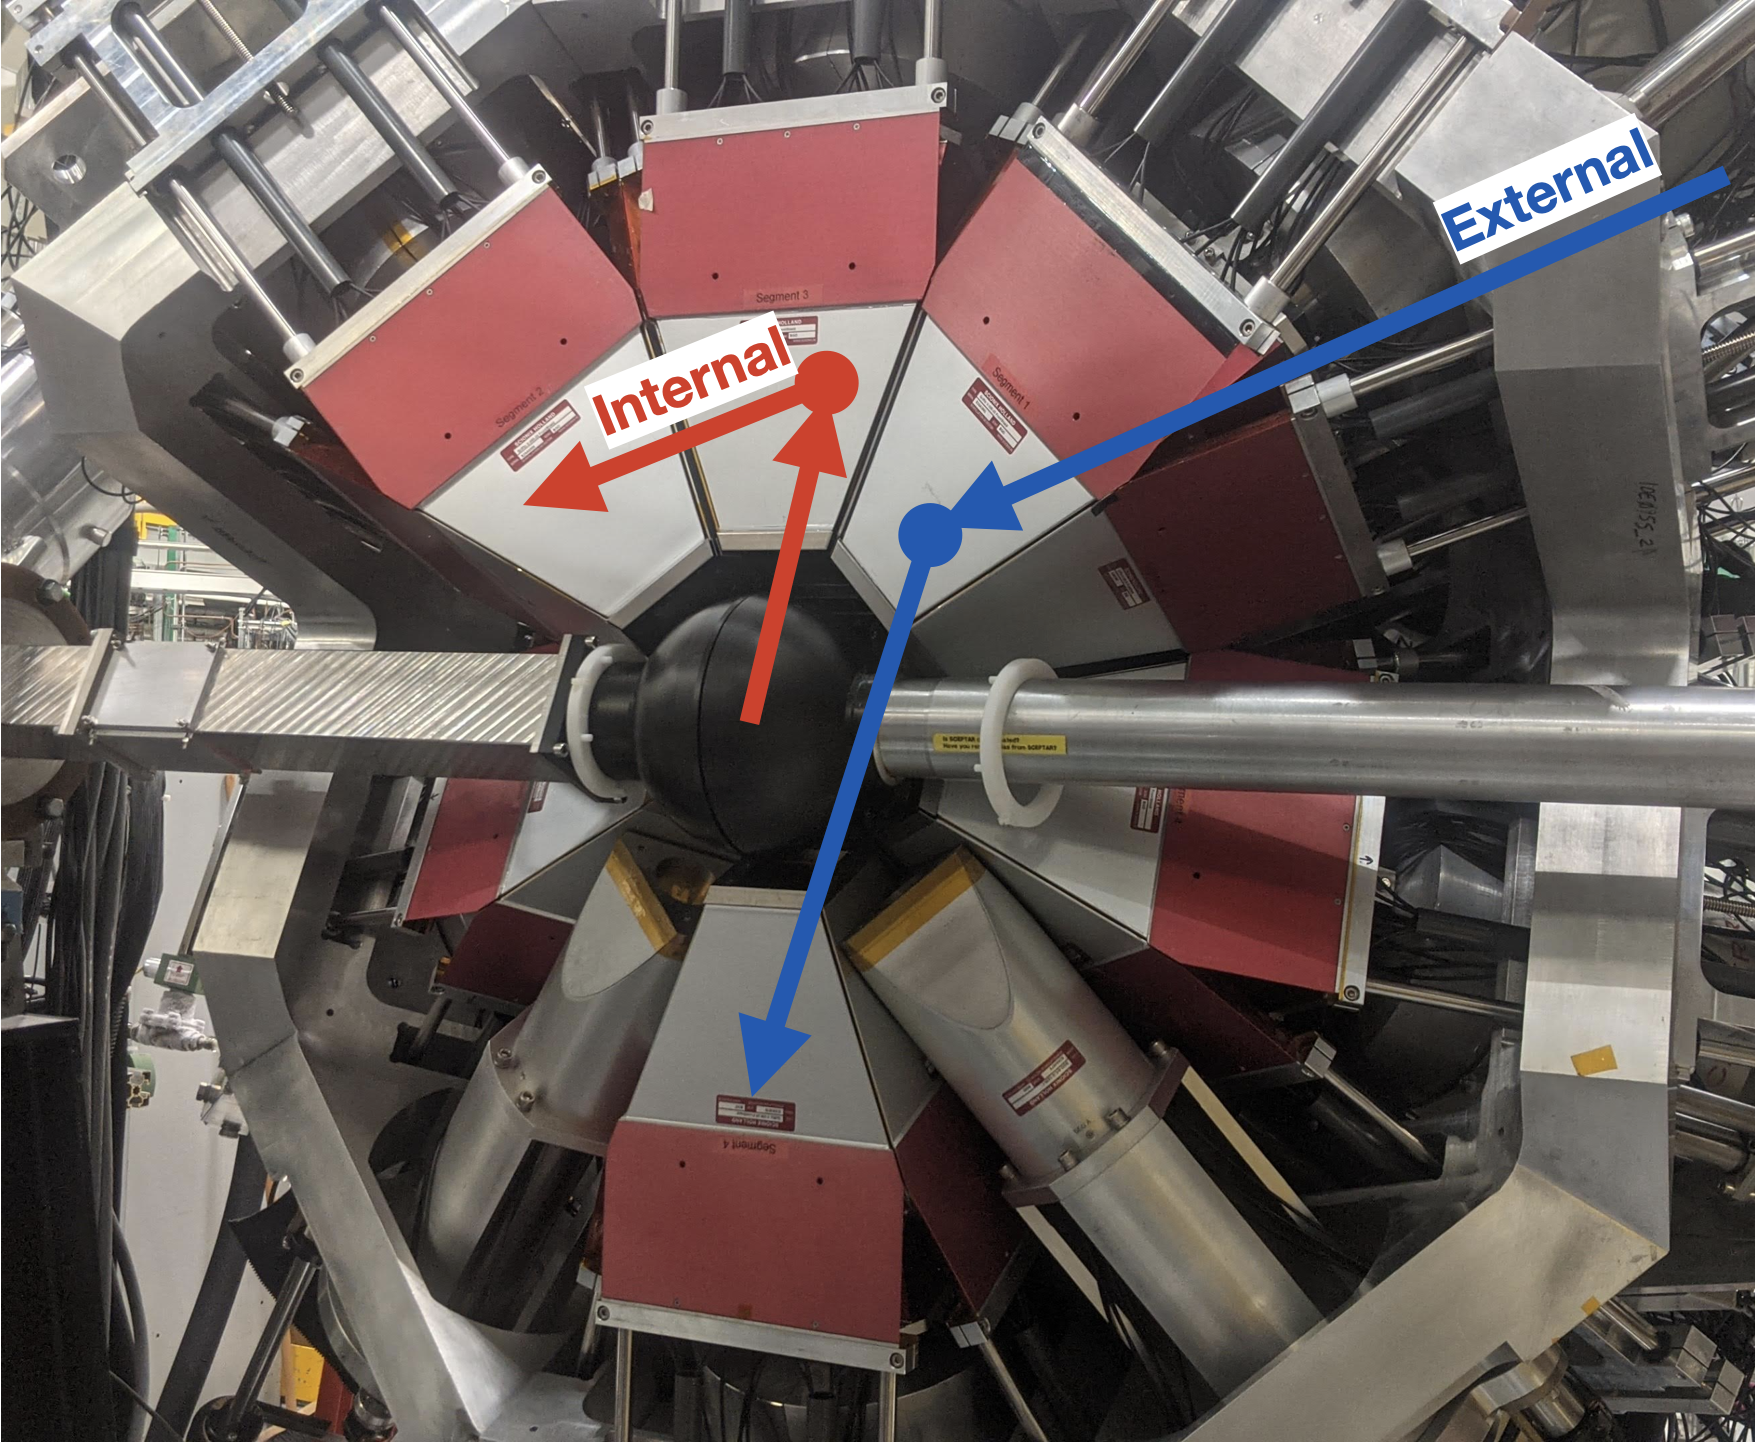
\includegraphics[width=0.95\textwidth]{compton_scatter_photo.png}
    \caption{Internal (red) vs external (blue) Compton-scatters in the GRIFFIN array. The vacuum chamber in the photo was not present during the $^{90}$Sr data collection.}
    \label{fig:compton_scatter_griffin_photo}
\end{figure}

\begin{figure}[htbp]
  \centering
  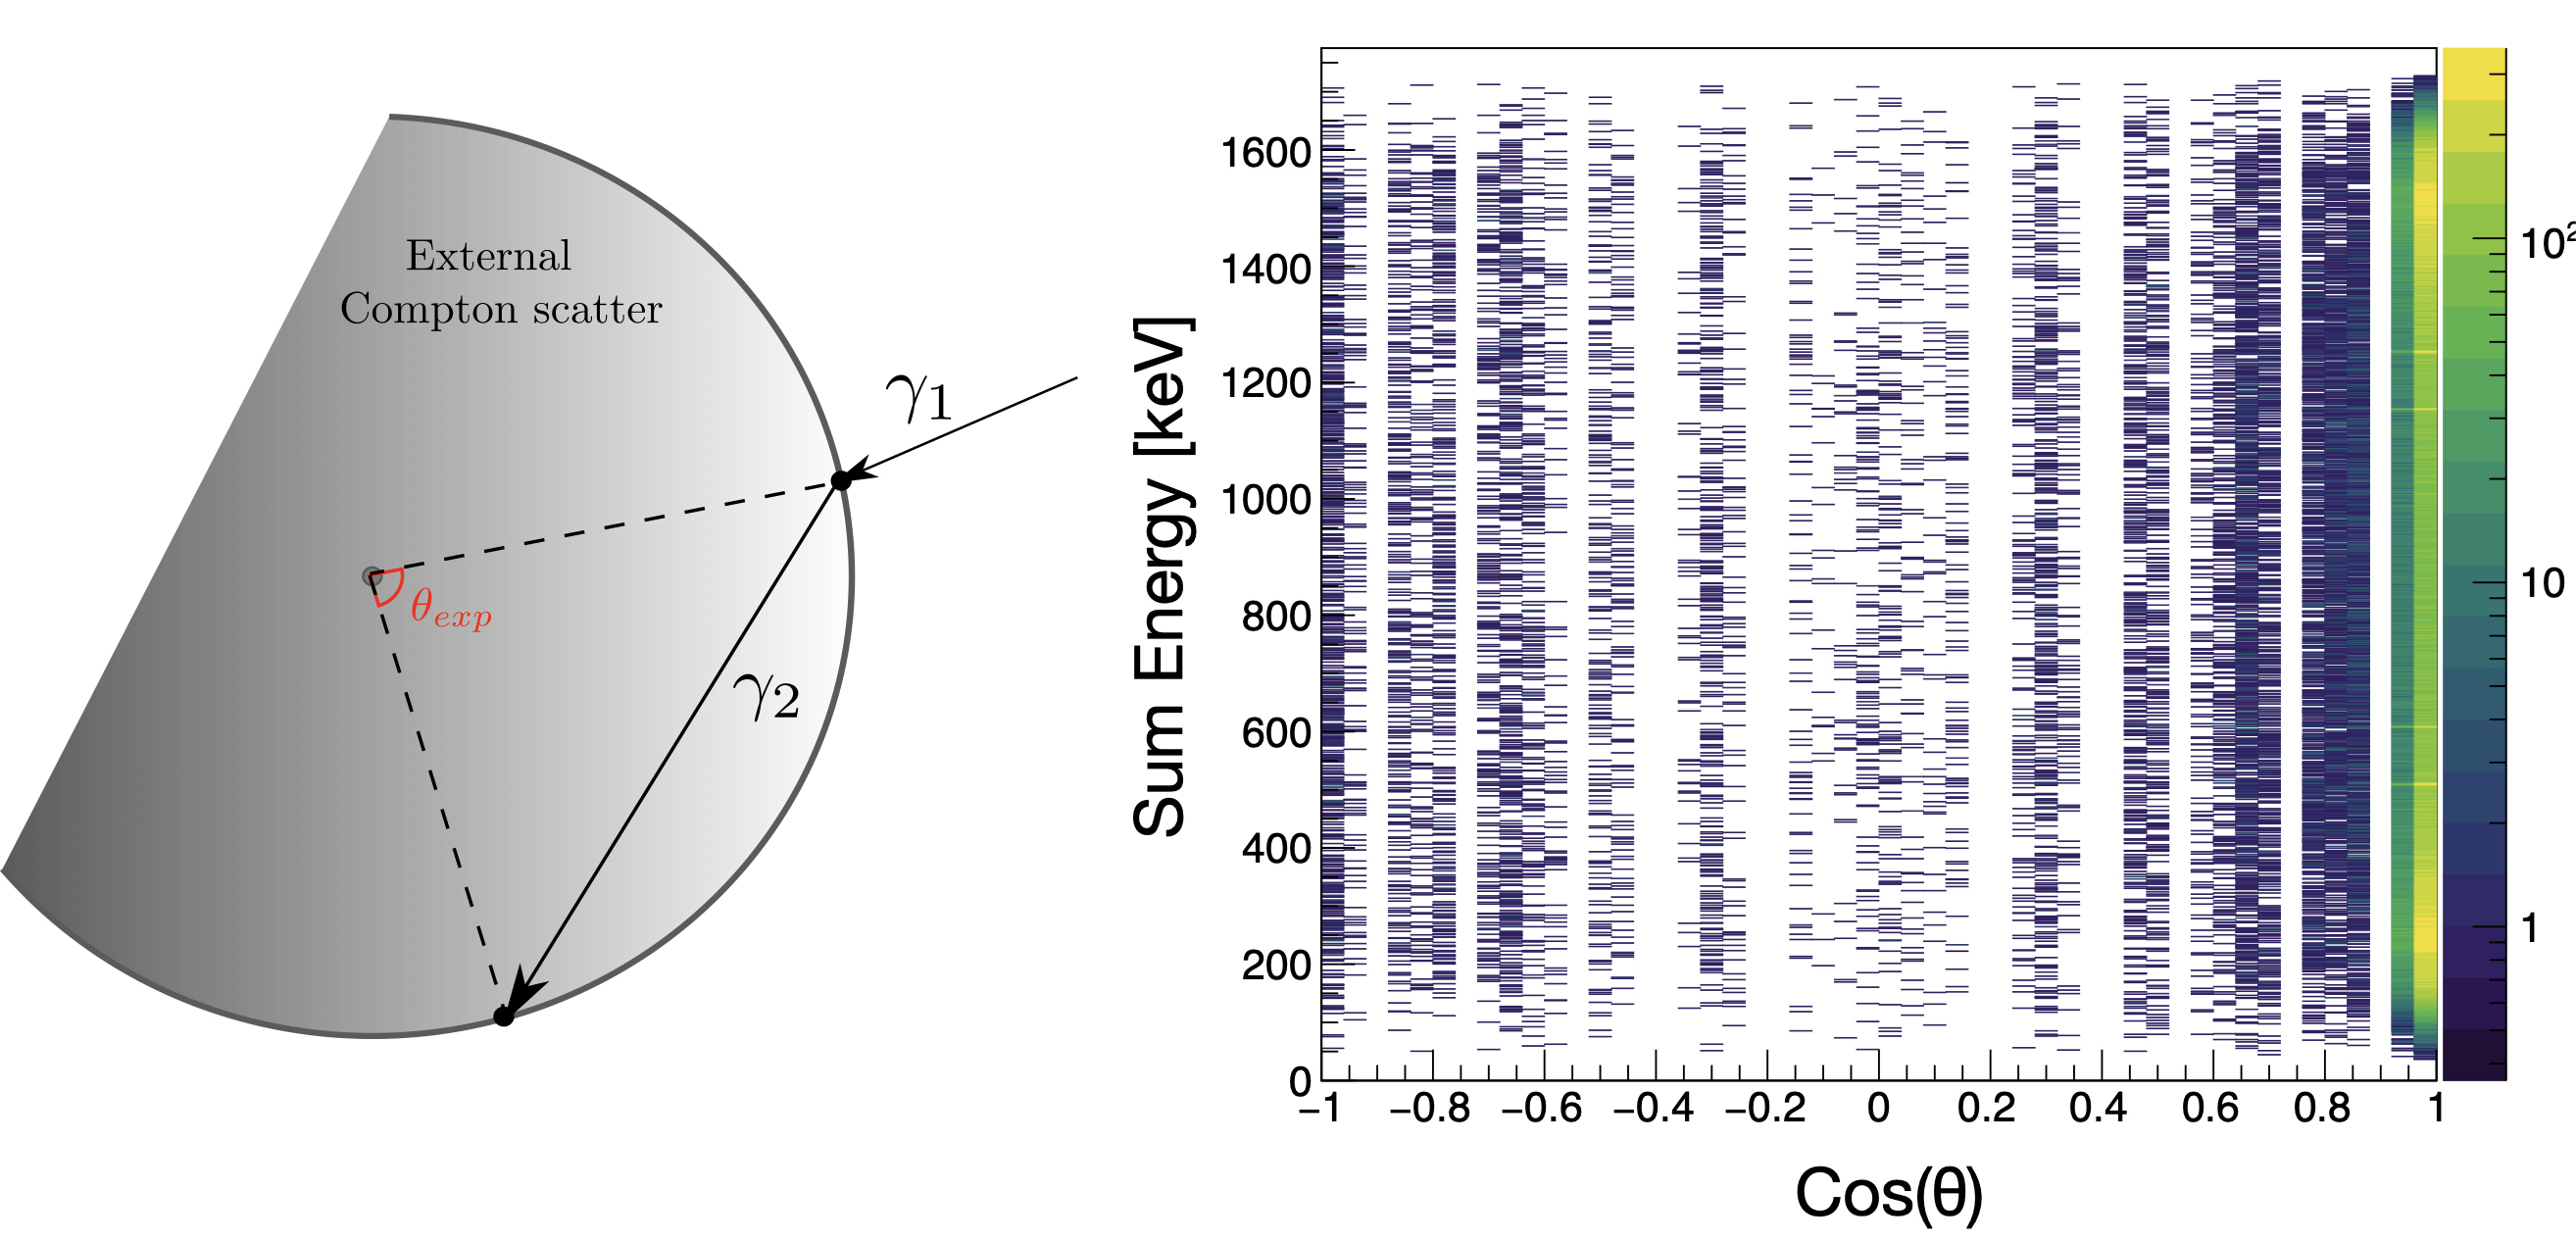
\includegraphics[width=0.95\textwidth]{external_compton_scatter.png}
  \caption{
    \textit{Left:} Schematic image of external Compton-scatter. The photon originates from outside the array and then scatters between detectors creating a multiplicity two event.
    \textit{Right:} Angular matrix created from 506 hours of $^{90}$Sr data gated on the Compton continuum.
  }
  \label{fig:external_compton_scatter_schematic}
\end{figure}

\begin{figure}[htbp]
  \centering
  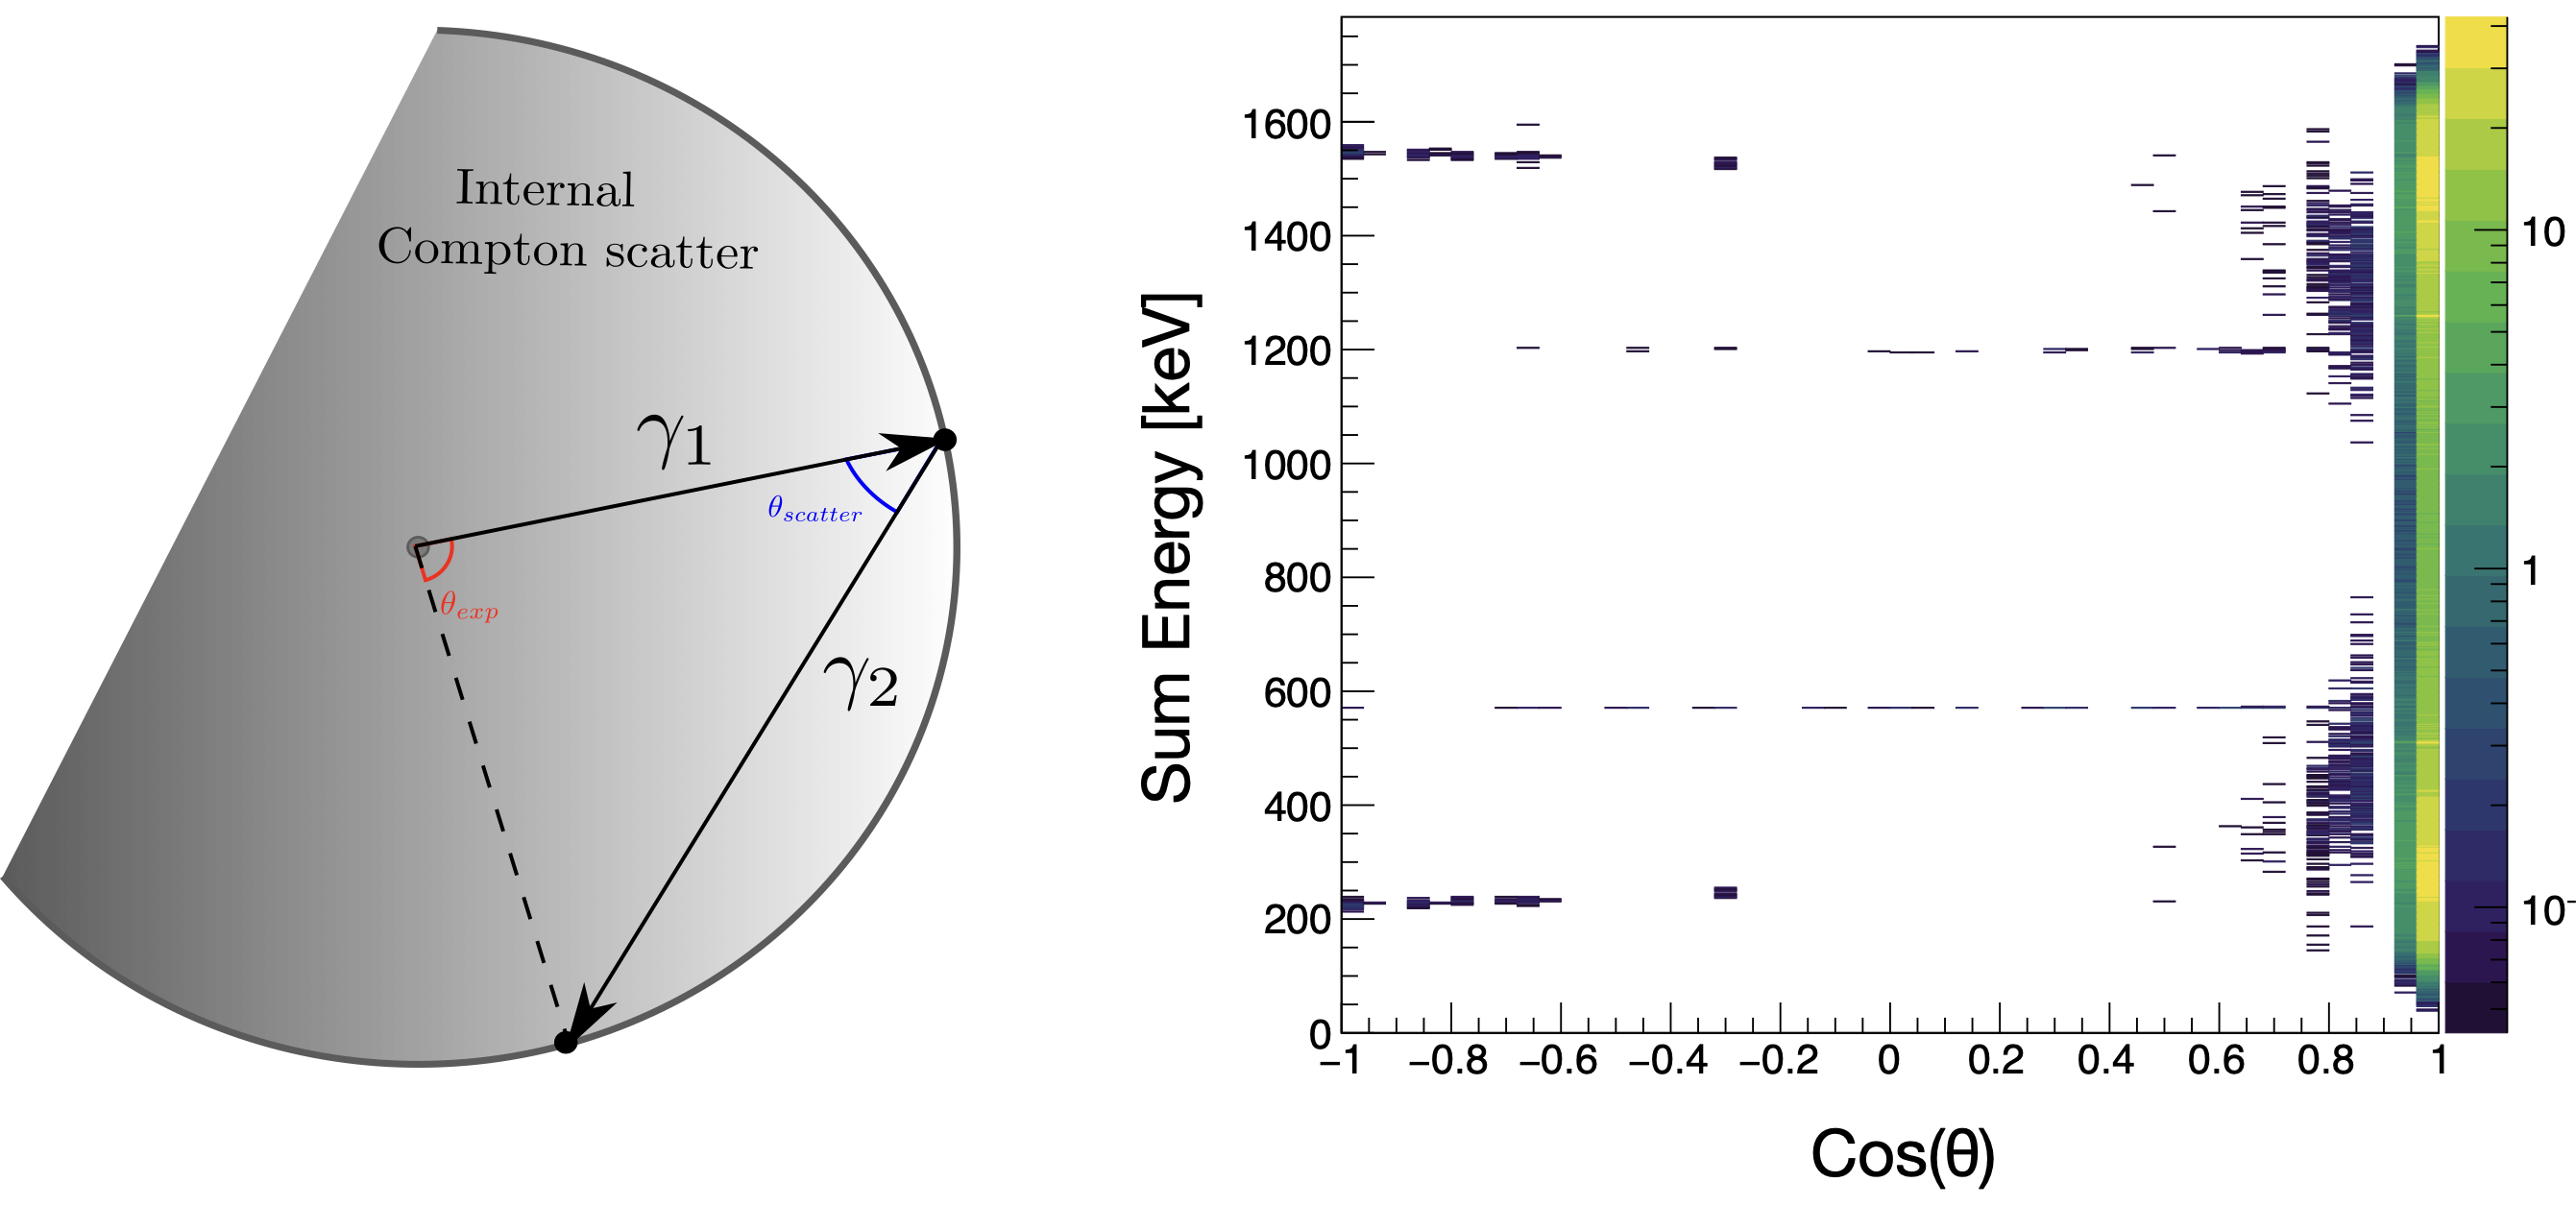
\includegraphics[width=0.95\textwidth]{internal_compton_scatter.png}
  \caption{
    \textit{Left:} Schematic image of internal Compton-scatter. The photon originates from the centre of the array and then scatters between detectors creating a multiplicity two event.
    \textit{Right:} Angular matrix created from 1 hour of $^{207}$Bi data gated on the 1770 keV peak.
  }
  \label{fig:internal_compton_scatter_schematic}
\end{figure}

\begin{figure}[htbp]
  \centering
  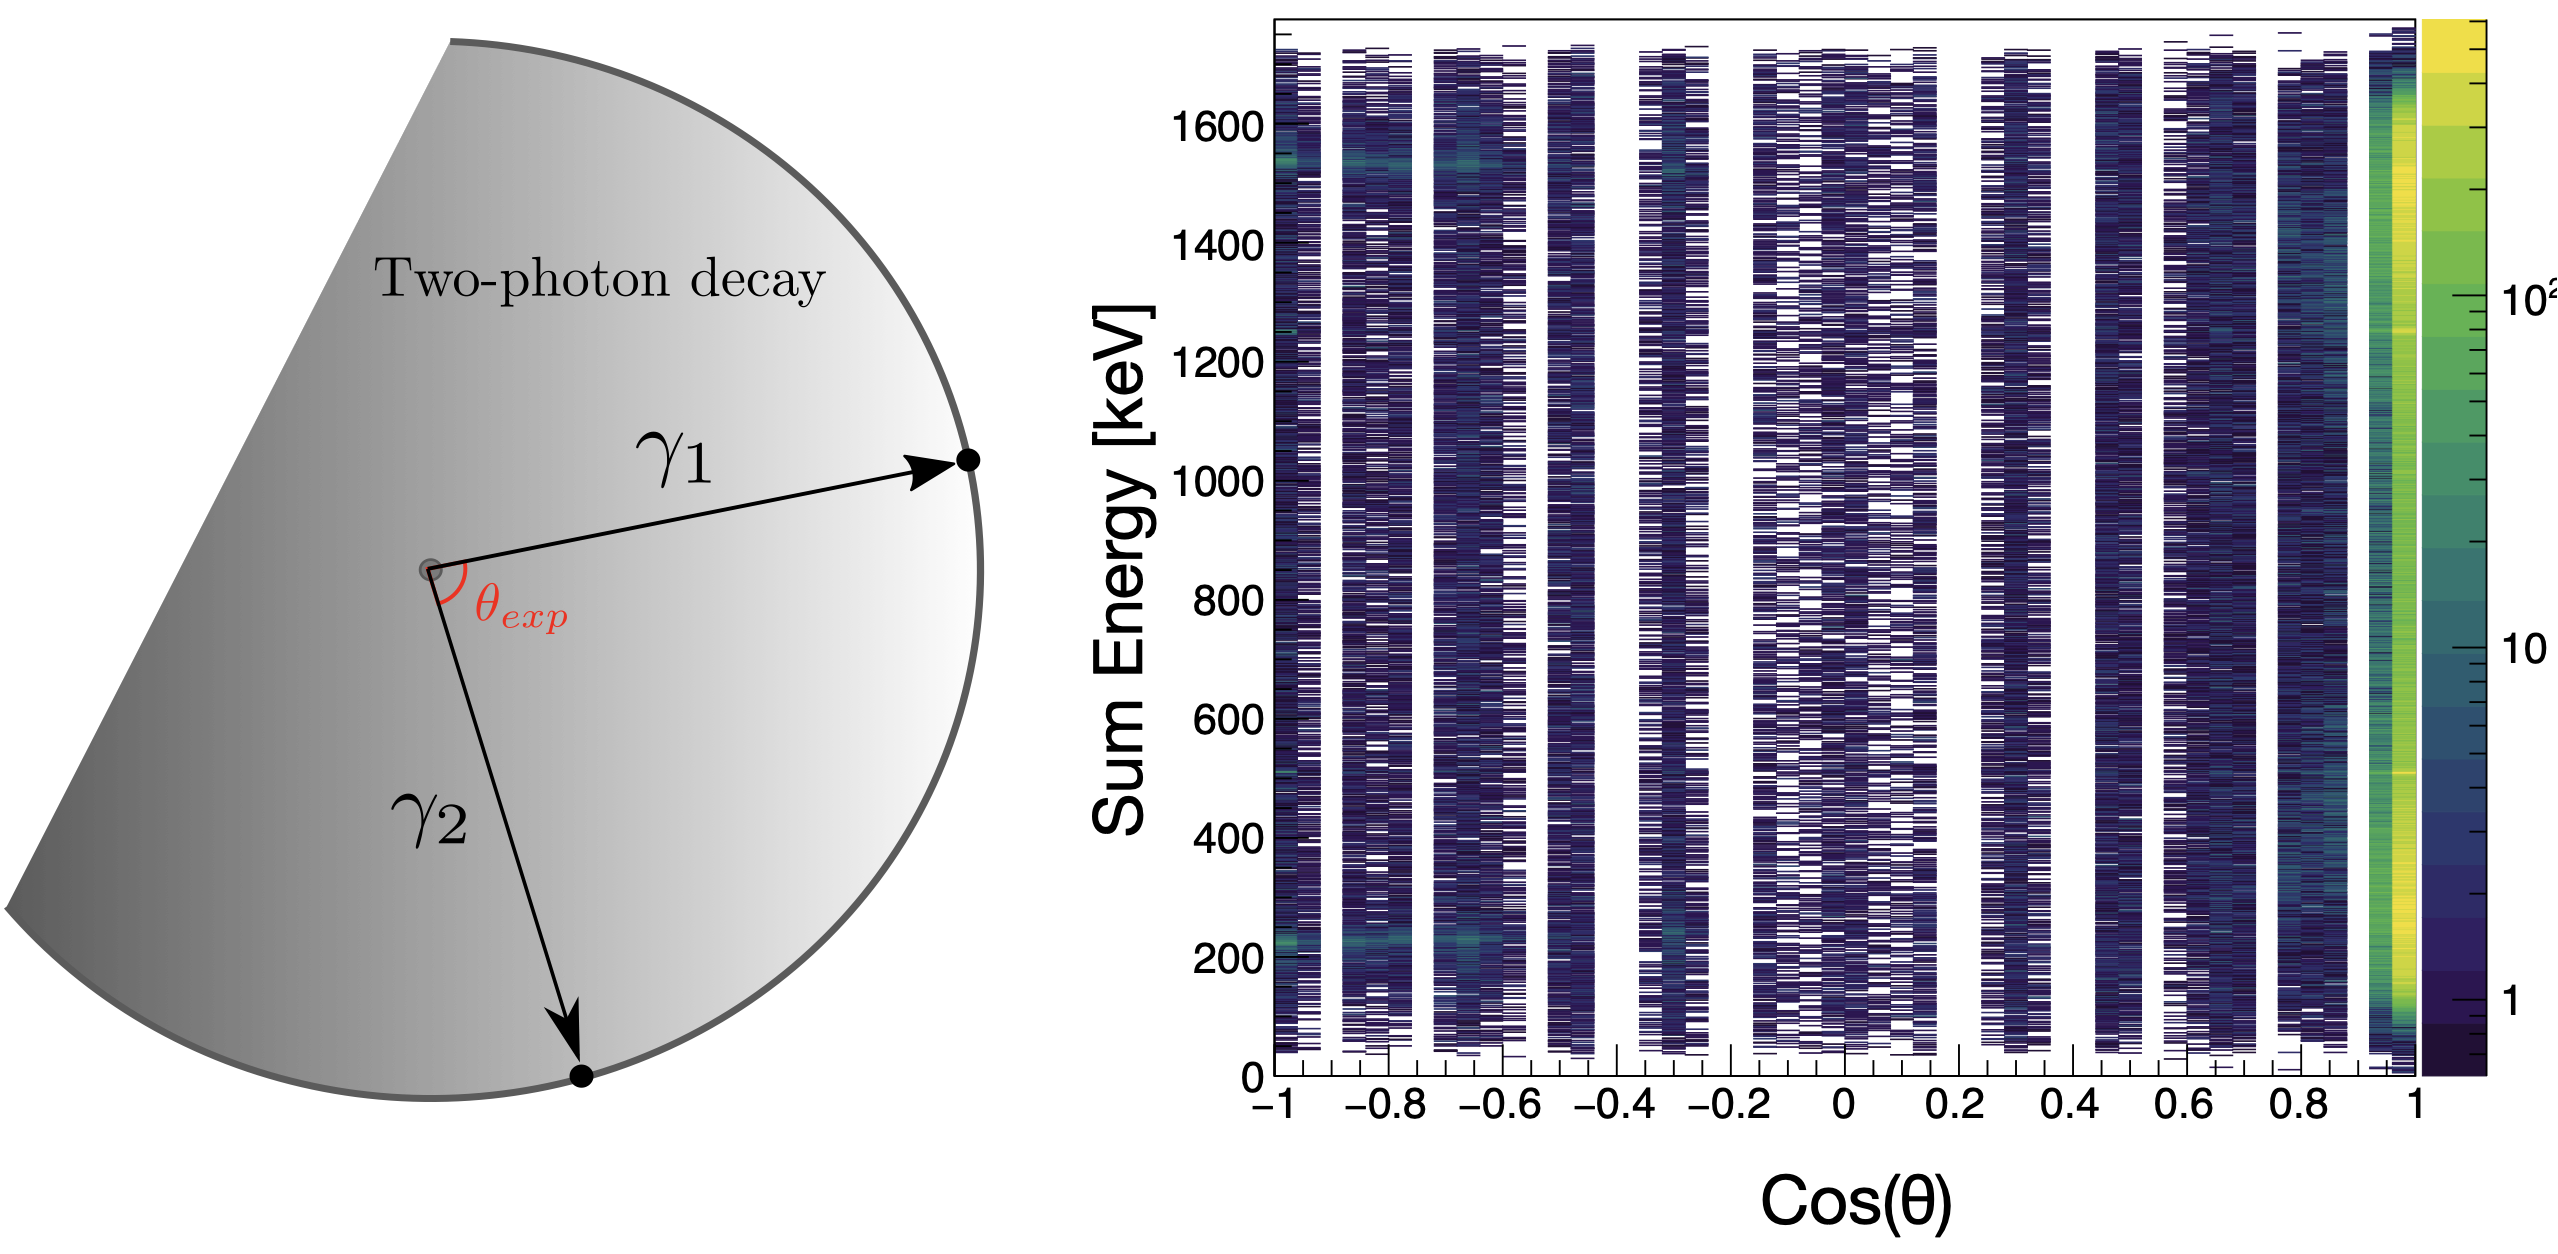
\includegraphics[width=0.95\textwidth]{two_photon_angular_correlation.png}
  \caption{
    \textit{Left:} Schematic image of two-photon decay. The two photons originate from the center of the array and both interact in different detectors creating a multiplicity two event.
    \textit{Right:} Angular matrix created from 506 hours of $^{90}$Sr data gated on the 1760 keV two-photon peak.
  }
  \label{fig:two_photon_angular_schematic}
\end{figure}

%------------------------------------------
\subsubsection{Simulation}
\label{sec:simulation}
%------------------------------------------
To better understand the data analysis procedure and hope to properly isolate two-photon events, Monte-Carlo simulations are being developed to model nuclear two-photon decay in GRIFFIN.
The simulations are being performed using GEANT4~\cite{allison_recent_2016} and a custom physics package to simulate competitive two-photon decay.
Natively GEANT4 does not have a physics library to simulate nuclear two-photon decay, so a custom physics library is in the process of being written; this, alongside a pre-existing GRIFFIN simulation package~\cite{v_bildstein_griffincollaborationdetectorsimulations_v10_2017} will allow a complete simulation campaign to be performed to better understand how two-photon events interact with GRIFFIN.

In its present state the two-photon physics library allows for fully competitive two-photon decay with user-tunable parameters to customize the decay for a variety of experimental cases.
The branching ratio of two-photon decay, the ratio of two-photon events to first order decays such as internal conversion or single gamma decay; the multipolarity of the decay, the ratio of dipole transitions to quadrupole transitions; and the mixing ratio of electric to magnetic dipoles are all tunable parameters that can be used to constrain experimental measurements and assist in the assignment of those values.
The simulation has been used to generate an angular matrix similar to \ref{fig:two_photon_angular_schematic} except only two-photon transitions were enabled, no other decay modes were allowed, shown in~\ref{fig:simulated_twophoton_angular_matrix}.
The two-photon physics have not been validated with the GRIFFIN simulation at this time, but they still provide a tool with which to help identify two-photon events present in the most recent dataset.

\begin{figure}[htbp]
  \centering
  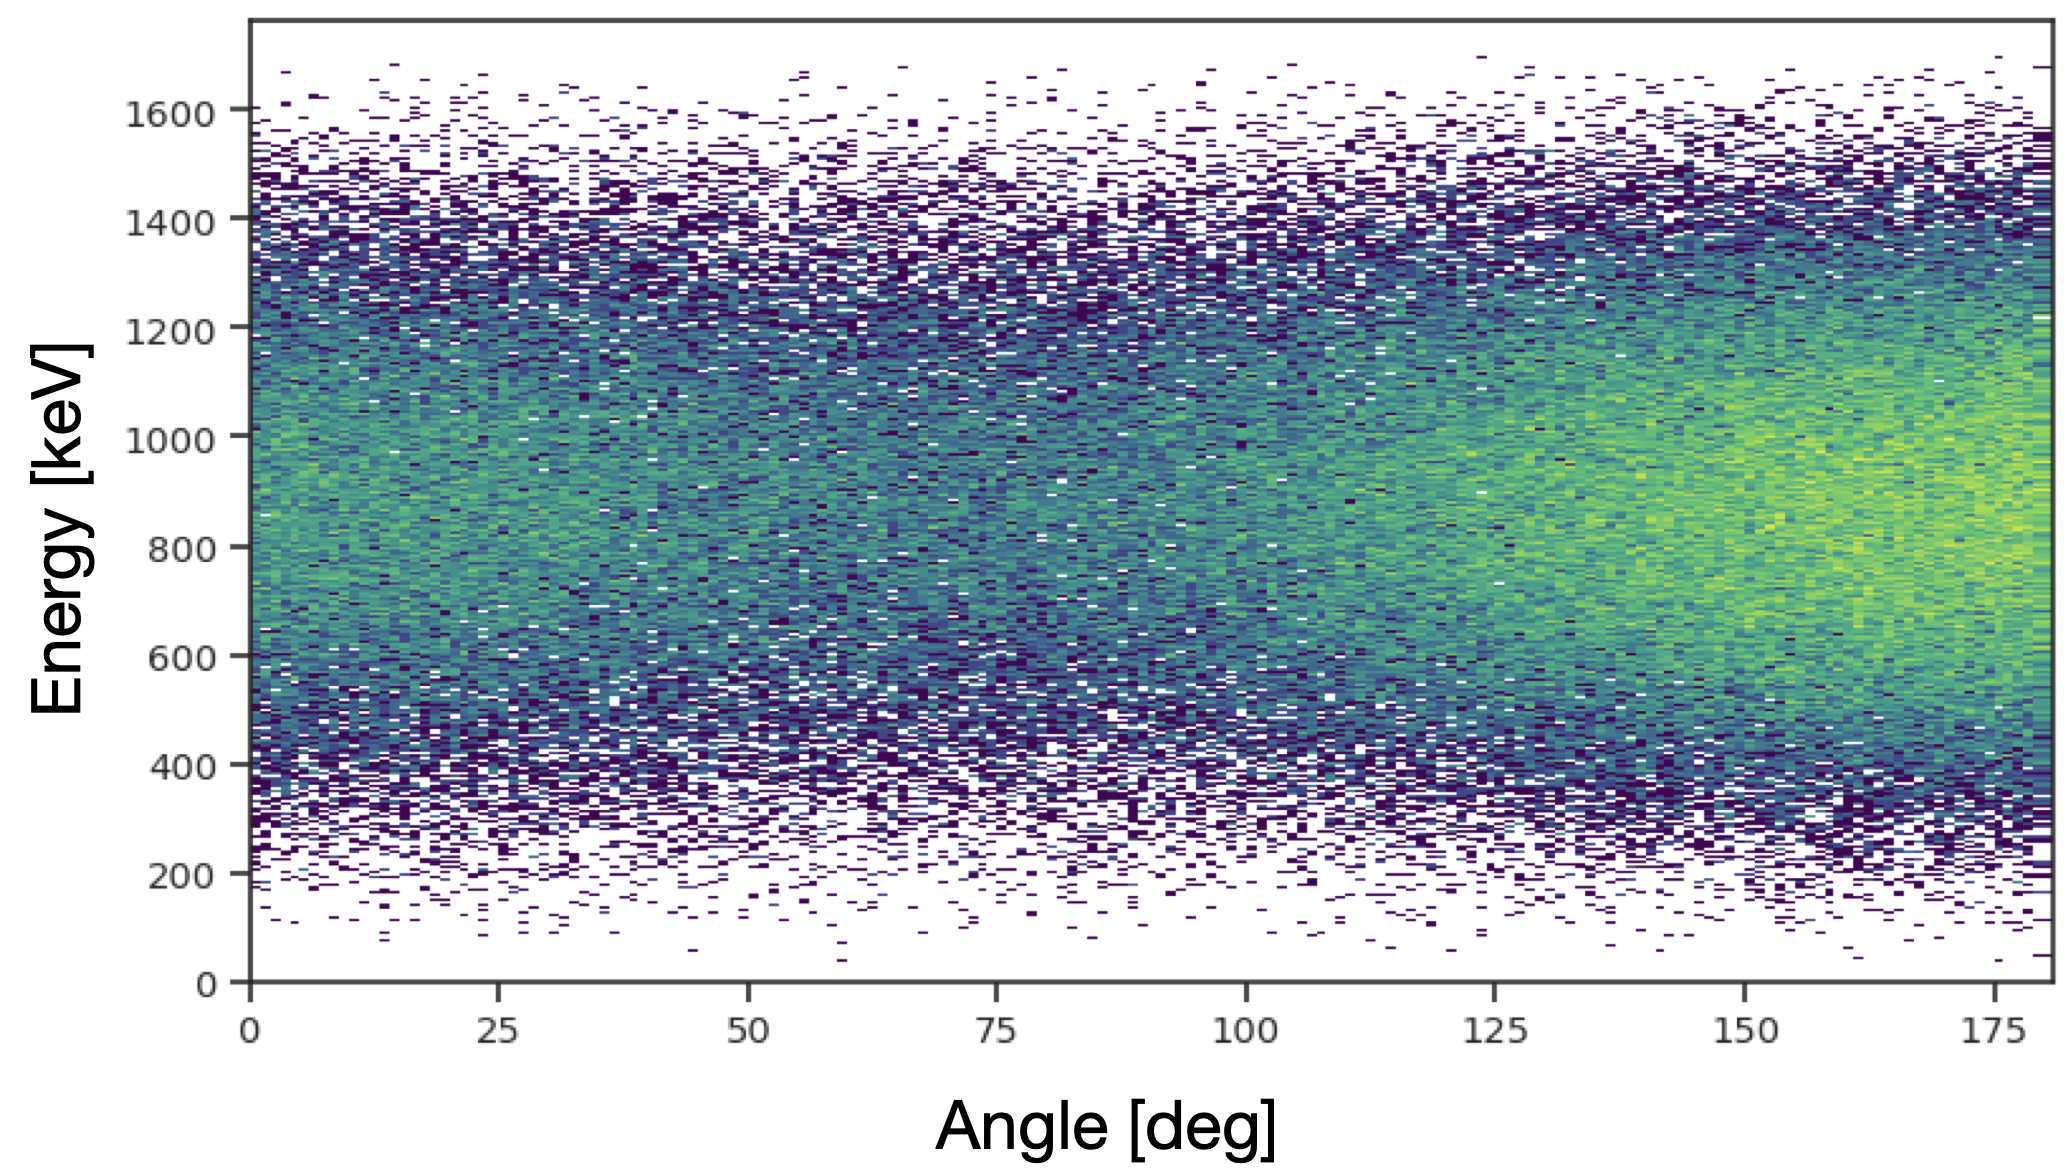
\includegraphics[width=0.95\textwidth]{simulated_twophoton_angular_matrix.png}
  \caption{Simulated two-photon angular matrix using the custom GEANT4 physics library where angle is the angle between the photons and energy is the energy of a single photon. This is not a matrix created from simulated GRIFFIN hits but the emitted distribution from a $^{90}$Y source.}
  \label{fig:simulated_twophoton_angular_matrix}
\end{figure}

%------------------------------------------
\subsubsection{Modeling Compton-scattering}
\label{sec:compton_scatter}
%------------------------------------------
With the reduction of Bremsstrahlung radiation through a redesign of the source itself, the most troublesome background the $^{214}$Bi $\beta^-$ decay.
The 1764 keV peak in the sum spectrum from $\gamma$-ray from $^{214}$Bi appears because of external Compton-scattering between detectors (see \ref{sec:angular_matrices}) and can appear as a two-photon event.
Since the energy-angle distribution of Compton scattering is well understood, this relationship can be mapped to the GRIFFIN experimental angle taking into account the finite detector opening angle and size.
The shaded area in~\ref{fig:compton_angle_mapping} denotes the scattering angles where an incident photon, incident from outside the array, interacts with one detector and scatters in such a way that it will not interact with a second detector based on the geometry of the GRIFFIN detectors. 
The non-shaded area shows the scattering angles that are accepted, the incident photon will interact with one detector and scatter into another, and could register as a two-photon event.


\begin{figure}[htbp]
  \centering
  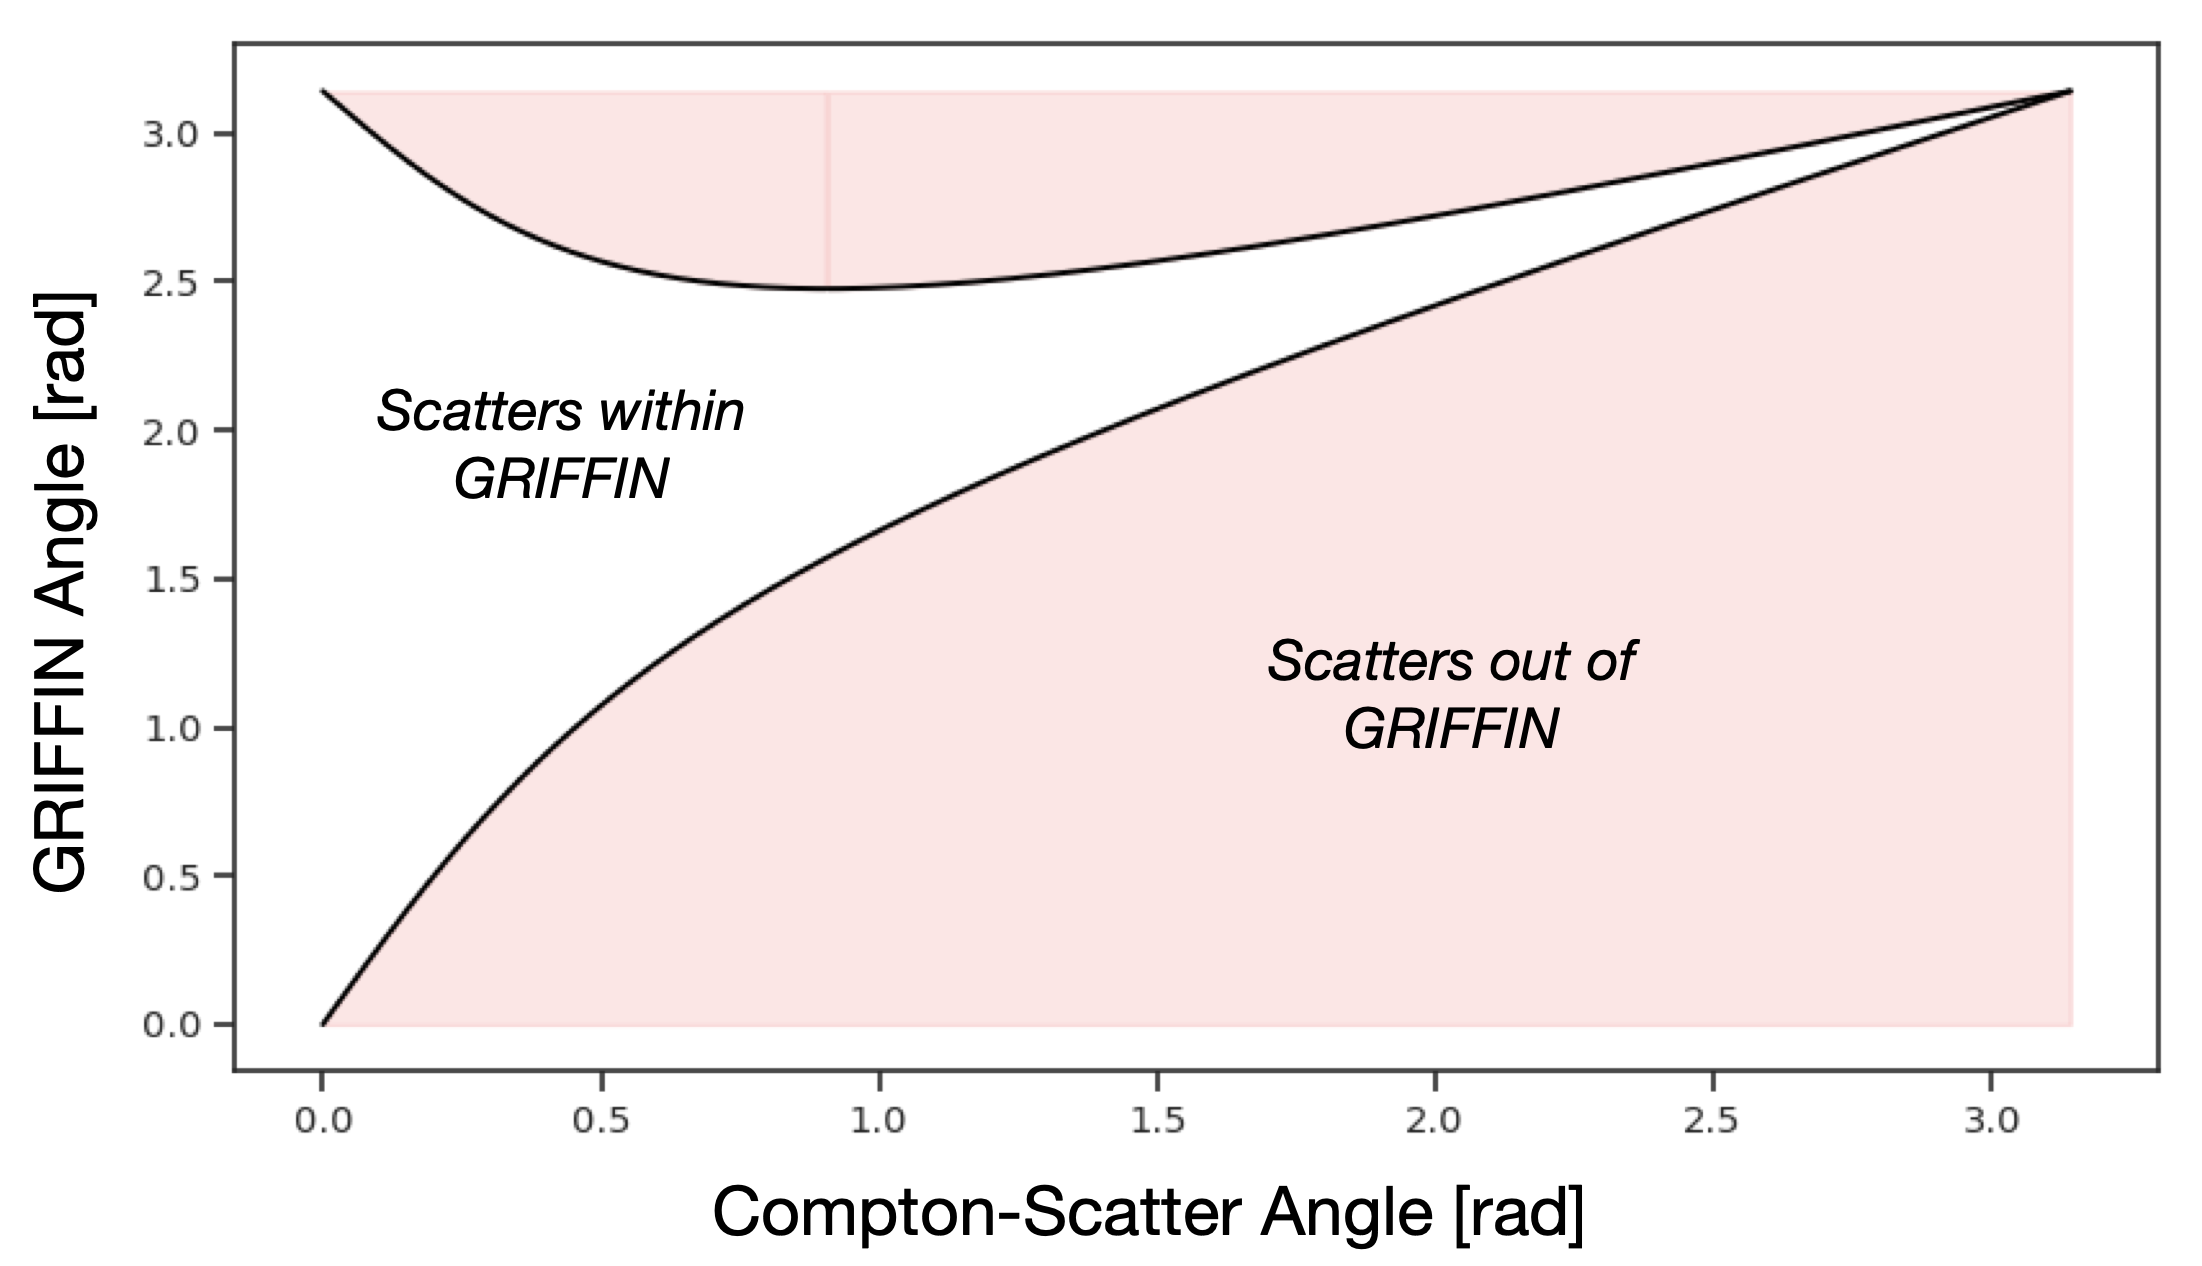
\includegraphics[width=0.95\textwidth]{compton_angle_mapping.png}
  \caption{Mapping of Compton-scatter angles to GRIFFIN centre of array angles for $\gamma$-rays originating from outside the array. The shaded areas denote an external Compton-scatter where the photon scatters away from the array and will not interact with a second detector, non-shaded areas show what Compton-scatters will show up as multiplicity two events in GRIFFIN.}
  \label{fig:compton_angle_mapping}
\end{figure}

Using the accepted GRIFFIN scattering angles, the Compton-scatter formula (see Section~\ref{sec:compton_scatter}) gives the energy-angle bands of photon energies that could be Compton-scatters rather than true two-photon events.
The bands are shown in~\ref{fig:simulation_data_comparison_with_compton_bands} as black and red bands on the simulated and collected energy-angle matrices respectively.
These bands support the observation of two-photon events because as the simulation shows the energy of the two-photon events are peaked around the middle of the energy range and extended minimally into the Compton-scattering bands. 
This can be used to further refine the selection of two-photon events and a general use algorithm is being developed to remove, or reconstruct, Compton-scatter events when filling a matrix. 
This algorithm is still in the development stage but should increase the peak-to-background ratio of a two-photon peak in a sum spectrum such as~\ref{fig:sum_spectrum_dec2019}.

\begin{figure}[htbp]
  \centering
  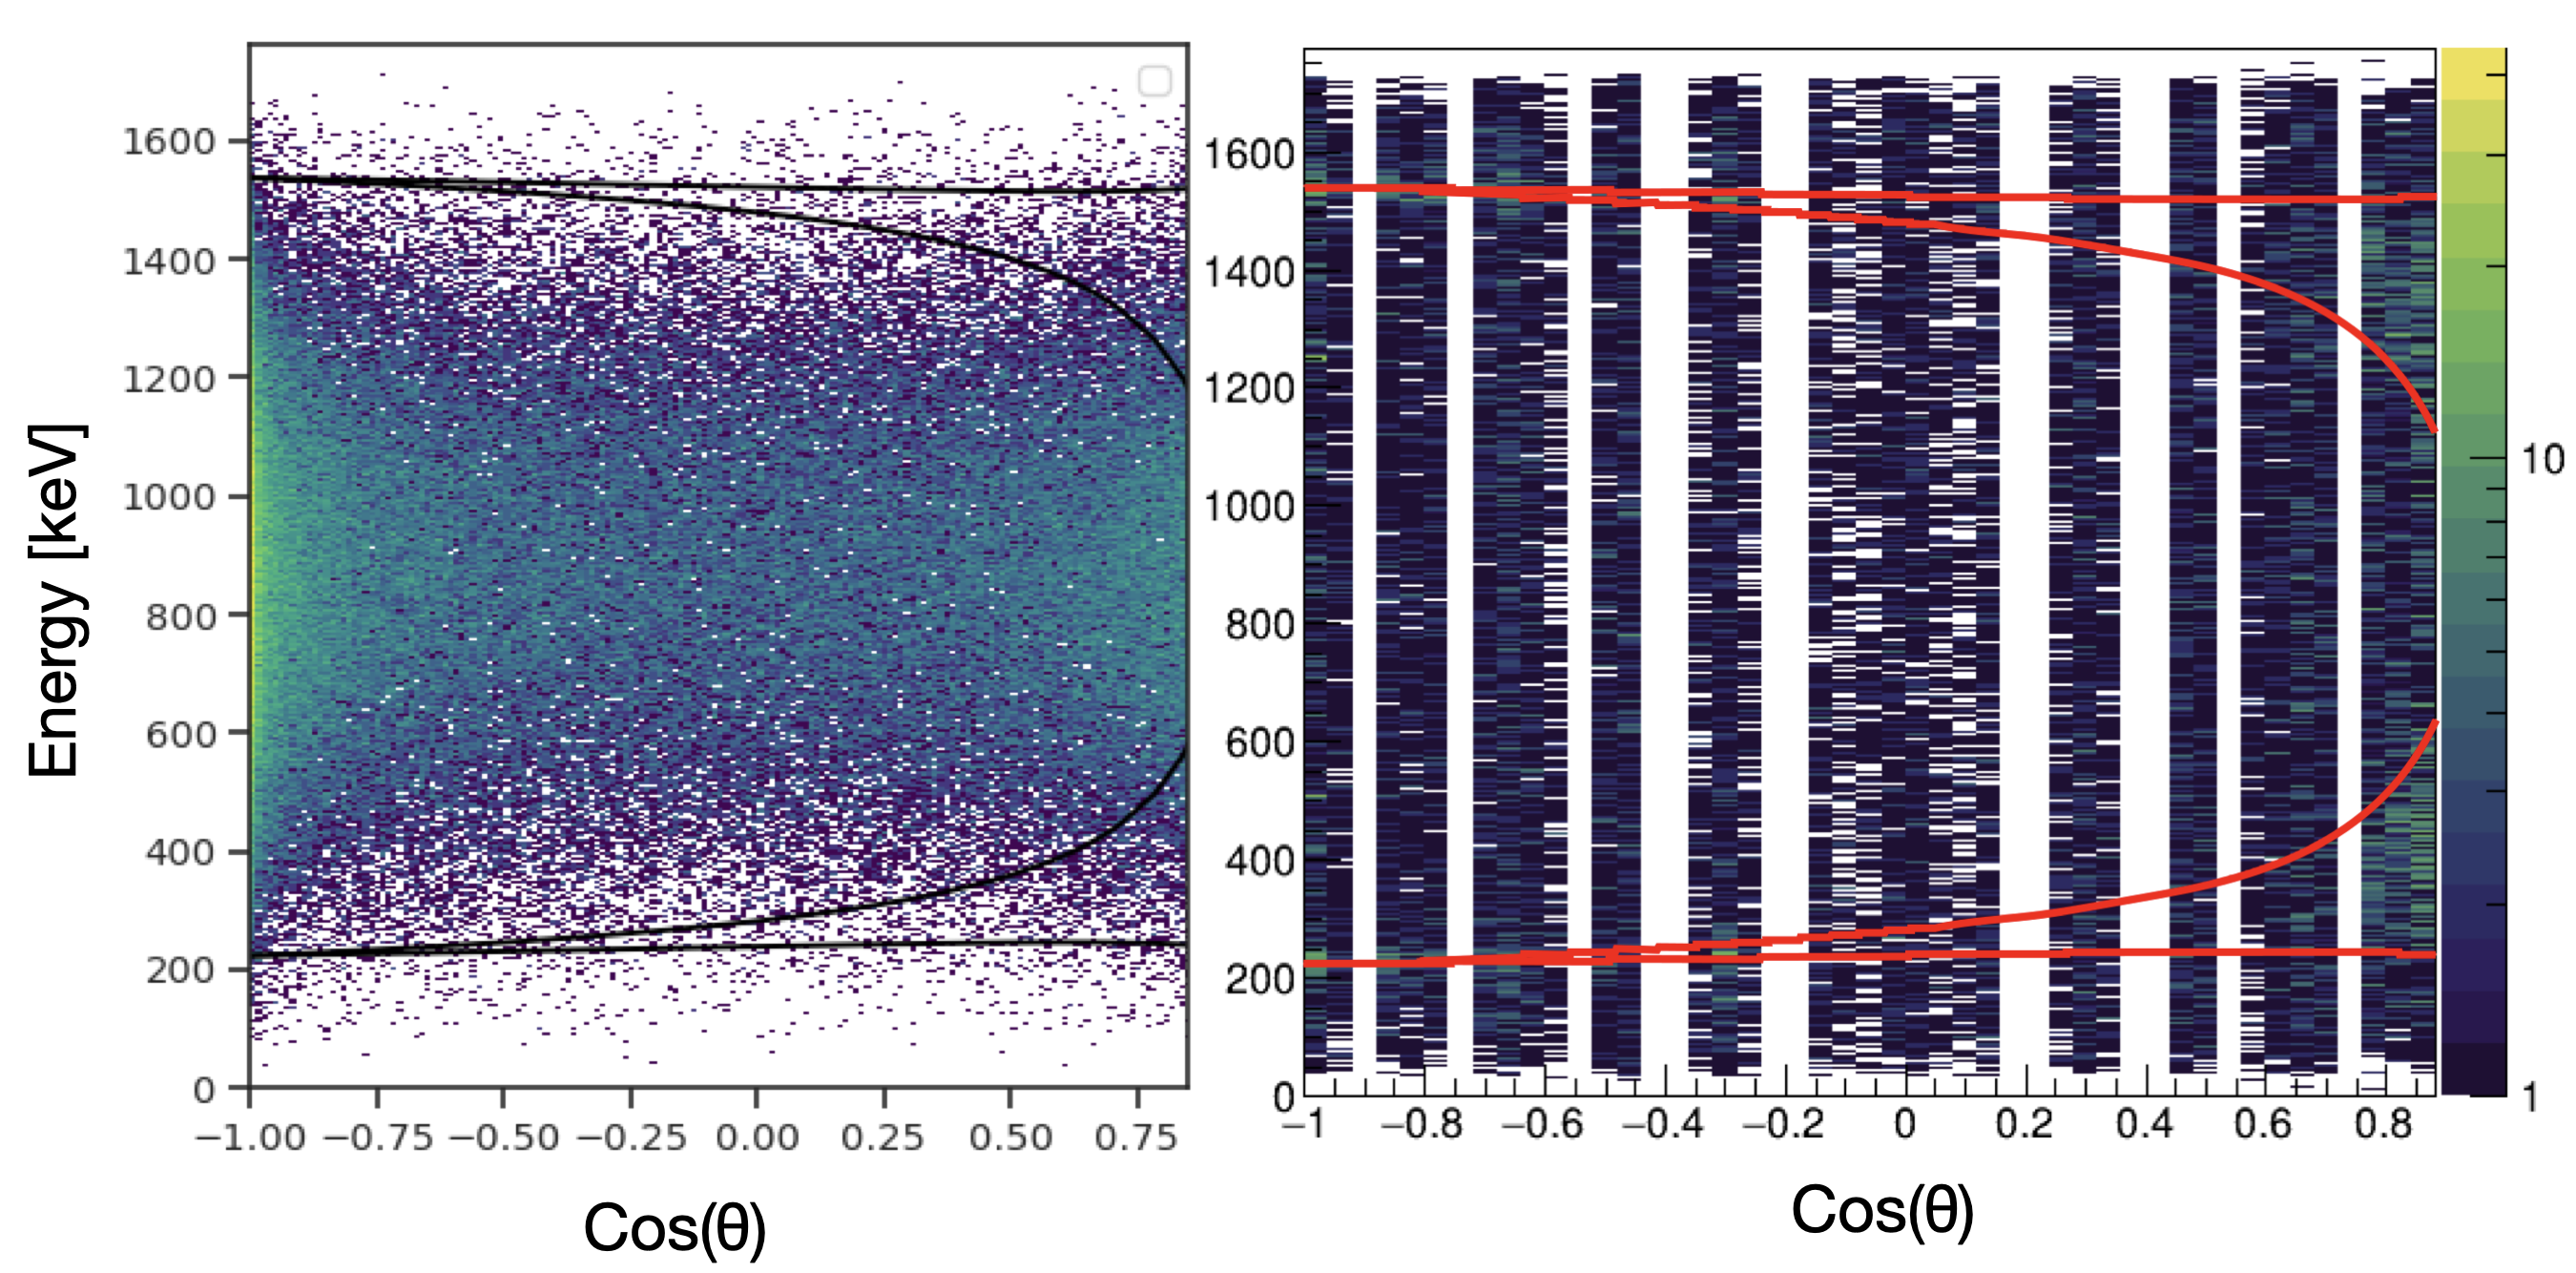
\includegraphics[width=0.95\textwidth]{simulation_vs_data_anglematrix_with_compton_bands.png}
  \caption{Comparison of simulated energy-angle matrix with the energy-angle matrix, gated on the two-photon peak, with Compton-scattering bands superimposed on both. Inter-clover scattering angles are not shown in the plot because the are ignored in the data analysis.  
    \textit{Left:} Simulated energy-angle matrix with Compton-scattering bands plotted in black. Any events between the bands is a possible Compton-scatter and can be vetoed in future histogram generation.
    \textit{Right:} $^{90}$Sr source energy-angle matrix with Compton-scattering bands plotted in red. Any events between the bands is a possible Compton-scatter and can be vetoed in future histogram generation.
  }
  \label{fig:simulation_data_comparison_with_compton_bands}
\end{figure}
%------------------------------------------
\end{document}
%------------------------------------------
